% Options for packages loaded elsewhere
\PassOptionsToPackage{unicode}{hyperref}
\PassOptionsToPackage{hyphens}{url}
%
\documentclass[
]{article}
\usepackage{lmodern}
\usepackage{amssymb,amsmath}
\usepackage{ifxetex,ifluatex}
\ifnum 0\ifxetex 1\fi\ifluatex 1\fi=0 % if pdftex
  \usepackage[T1]{fontenc}
  \usepackage[utf8]{inputenc}
  \usepackage{textcomp} % provide euro and other symbols
\else % if luatex or xetex
  \usepackage{unicode-math}
  \defaultfontfeatures{Scale=MatchLowercase}
  \defaultfontfeatures[\rmfamily]{Ligatures=TeX,Scale=1}
\fi
% Use upquote if available, for straight quotes in verbatim environments
\IfFileExists{upquote.sty}{\usepackage{upquote}}{}
\IfFileExists{microtype.sty}{% use microtype if available
  \usepackage[]{microtype}
  \UseMicrotypeSet[protrusion]{basicmath} % disable protrusion for tt fonts
}{}
\makeatletter
\@ifundefined{KOMAClassName}{% if non-KOMA class
  \IfFileExists{parskip.sty}{%
    \usepackage{parskip}
  }{% else
    \setlength{\parindent}{0pt}
    \setlength{\parskip}{6pt plus 2pt minus 1pt}}
}{% if KOMA class
  \KOMAoptions{parskip=half}}
\makeatother
\usepackage{xcolor}
\IfFileExists{xurl.sty}{\usepackage{xurl}}{} % add URL line breaks if available
\IfFileExists{bookmark.sty}{\usepackage{bookmark}}{\usepackage{hyperref}}
\hypersetup{
  pdftitle={Main: Facial Expression Recognition Framework},
  pdfauthor={Group 1: Kristen Akey, Levi Lee, Yiran Lin, Hanyi Yang, Wen Yin},
  hidelinks,
  pdfcreator={LaTeX via pandoc}}
\urlstyle{same} % disable monospaced font for URLs
\usepackage[margin=1in]{geometry}
\usepackage{color}
\usepackage{fancyvrb}
\newcommand{\VerbBar}{|}
\newcommand{\VERB}{\Verb[commandchars=\\\{\}]}
\DefineVerbatimEnvironment{Highlighting}{Verbatim}{commandchars=\\\{\}}
% Add ',fontsize=\small' for more characters per line
\usepackage{framed}
\definecolor{shadecolor}{RGB}{248,248,248}
\newenvironment{Shaded}{\begin{snugshade}}{\end{snugshade}}
\newcommand{\AlertTok}[1]{\textcolor[rgb]{0.94,0.16,0.16}{#1}}
\newcommand{\AnnotationTok}[1]{\textcolor[rgb]{0.56,0.35,0.01}{\textbf{\textit{#1}}}}
\newcommand{\AttributeTok}[1]{\textcolor[rgb]{0.77,0.63,0.00}{#1}}
\newcommand{\BaseNTok}[1]{\textcolor[rgb]{0.00,0.00,0.81}{#1}}
\newcommand{\BuiltInTok}[1]{#1}
\newcommand{\CharTok}[1]{\textcolor[rgb]{0.31,0.60,0.02}{#1}}
\newcommand{\CommentTok}[1]{\textcolor[rgb]{0.56,0.35,0.01}{\textit{#1}}}
\newcommand{\CommentVarTok}[1]{\textcolor[rgb]{0.56,0.35,0.01}{\textbf{\textit{#1}}}}
\newcommand{\ConstantTok}[1]{\textcolor[rgb]{0.00,0.00,0.00}{#1}}
\newcommand{\ControlFlowTok}[1]{\textcolor[rgb]{0.13,0.29,0.53}{\textbf{#1}}}
\newcommand{\DataTypeTok}[1]{\textcolor[rgb]{0.13,0.29,0.53}{#1}}
\newcommand{\DecValTok}[1]{\textcolor[rgb]{0.00,0.00,0.81}{#1}}
\newcommand{\DocumentationTok}[1]{\textcolor[rgb]{0.56,0.35,0.01}{\textbf{\textit{#1}}}}
\newcommand{\ErrorTok}[1]{\textcolor[rgb]{0.64,0.00,0.00}{\textbf{#1}}}
\newcommand{\ExtensionTok}[1]{#1}
\newcommand{\FloatTok}[1]{\textcolor[rgb]{0.00,0.00,0.81}{#1}}
\newcommand{\FunctionTok}[1]{\textcolor[rgb]{0.00,0.00,0.00}{#1}}
\newcommand{\ImportTok}[1]{#1}
\newcommand{\InformationTok}[1]{\textcolor[rgb]{0.56,0.35,0.01}{\textbf{\textit{#1}}}}
\newcommand{\KeywordTok}[1]{\textcolor[rgb]{0.13,0.29,0.53}{\textbf{#1}}}
\newcommand{\NormalTok}[1]{#1}
\newcommand{\OperatorTok}[1]{\textcolor[rgb]{0.81,0.36,0.00}{\textbf{#1}}}
\newcommand{\OtherTok}[1]{\textcolor[rgb]{0.56,0.35,0.01}{#1}}
\newcommand{\PreprocessorTok}[1]{\textcolor[rgb]{0.56,0.35,0.01}{\textit{#1}}}
\newcommand{\RegionMarkerTok}[1]{#1}
\newcommand{\SpecialCharTok}[1]{\textcolor[rgb]{0.00,0.00,0.00}{#1}}
\newcommand{\SpecialStringTok}[1]{\textcolor[rgb]{0.31,0.60,0.02}{#1}}
\newcommand{\StringTok}[1]{\textcolor[rgb]{0.31,0.60,0.02}{#1}}
\newcommand{\VariableTok}[1]{\textcolor[rgb]{0.00,0.00,0.00}{#1}}
\newcommand{\VerbatimStringTok}[1]{\textcolor[rgb]{0.31,0.60,0.02}{#1}}
\newcommand{\WarningTok}[1]{\textcolor[rgb]{0.56,0.35,0.01}{\textbf{\textit{#1}}}}
\usepackage{graphicx,grffile}
\makeatletter
\def\maxwidth{\ifdim\Gin@nat@width>\linewidth\linewidth\else\Gin@nat@width\fi}
\def\maxheight{\ifdim\Gin@nat@height>\textheight\textheight\else\Gin@nat@height\fi}
\makeatother
% Scale images if necessary, so that they will not overflow the page
% margins by default, and it is still possible to overwrite the defaults
% using explicit options in \includegraphics[width, height, ...]{}
\setkeys{Gin}{width=\maxwidth,height=\maxheight,keepaspectratio}
% Set default figure placement to htbp
\makeatletter
\def\fps@figure{htbp}
\makeatother
\setlength{\emergencystretch}{3em} % prevent overfull lines
\providecommand{\tightlist}{%
  \setlength{\itemsep}{0pt}\setlength{\parskip}{0pt}}
\setcounter{secnumdepth}{-\maxdimen} % remove section numbering

\title{Main: Facial Expression Recognition Framework}
\author{Group 1: Kristen Akey, Levi Lee, Yiran Lin, Hanyi Yang, Wen Yin}
\date{}

\begin{document}
\maketitle

\hypertarget{introduction-objective}{%
\section{Introduction / Objective}\label{introduction-objective}}

\hypertarget{baseline-modelproposed-model}{%
\section{Baseline Model/Proposed
Model}\label{baseline-modelproposed-model}}

\hypertarget{results}{%
\section{Results}\label{results}}

\hypertarget{analysis}{%
\section{Analysis}\label{analysis}}

In your final repo, there should be an R markdown file that organizes
\textbf{all computational steps} for evaluating your proposed Facial
Expression Recognition framework.

This file is currently a template for running evaluation experiments.
You should update it according to your codes but following precisely the
same structure.

\hypertarget{step-0-set-work-directories}{%
\subsubsection{Step 0 set work
directories}\label{step-0-set-work-directories}}

\begin{Shaded}
\begin{Highlighting}[]
\KeywordTok{set.seed}\NormalTok{(}\DecValTok{2020}\NormalTok{)}
\KeywordTok{setwd}\NormalTok{(}\StringTok{"~/GitHub/Fall2020-Project3-group1/doc"}\NormalTok{)}


\CommentTok{# change the working directory as needed}
\CommentTok{# if someone can make this a relative path, that would be great!!! }
\end{Highlighting}
\end{Shaded}

Provide directories for training images. Training images and Training
fiducial points will be in different subfolders.

\begin{Shaded}
\begin{Highlighting}[]
\CommentTok{# change the directory of the data to where it's stored in your local drive as needed}

\CommentTok{# train_dir <- "../data/train_set/" # This will be modified for different data sets.}

\NormalTok{train_dir <-}\StringTok{ "~/train_set/"}


\NormalTok{train_image_dir <-}\StringTok{ }\KeywordTok{paste}\NormalTok{(train_dir, }\StringTok{"images/"}\NormalTok{, }\DataTypeTok{sep=}\StringTok{""}\NormalTok{)}
\NormalTok{train_pt_dir <-}\StringTok{ }\KeywordTok{paste}\NormalTok{(train_dir,  }\StringTok{"points/"}\NormalTok{, }\DataTypeTok{sep=}\StringTok{""}\NormalTok{)}
\NormalTok{train_label_path <-}\StringTok{ }\KeywordTok{paste}\NormalTok{(train_dir, }\StringTok{"label.csv"}\NormalTok{, }\DataTypeTok{sep=}\StringTok{""}\NormalTok{) }
\end{Highlighting}
\end{Shaded}

\hypertarget{step-1-set-up-controls-for-evaluation-experiments.}{%
\subsubsection{Step 1: set up controls for evaluation
experiments.}\label{step-1-set-up-controls-for-evaluation-experiments.}}

In this chunk, we have a set of controls for the evaluation experiments.

\begin{itemize}
\tightlist
\item
  (T/F) cross-validation on the training set
\item
  (T/F) reweighting the samples for training set
\item
  (number) K, the number of CV folds
\item
  (T/F) process features for training set
\item
  (T/F) run evaluation on an independent test set
\item
  (T/F) process features for test set
\end{itemize}

\begin{Shaded}
\begin{Highlighting}[]
\NormalTok{K <-}\StringTok{ }\DecValTok{5}  \CommentTok{# number of CV folds}

\NormalTok{run.fudicial.list <-}\StringTok{ }\OtherTok{FALSE}
\NormalTok{run.feature.train <-}\StringTok{ }\OtherTok{FALSE} \CommentTok{# process features for training set}
\NormalTok{run.feature.test <-}\StringTok{ }\OtherTok{FALSE} \CommentTok{# process features for test set}
\NormalTok{sample.reweight <-}\StringTok{ }\OtherTok{TRUE} \CommentTok{# run sample reweighting in model training}

\NormalTok{run.cv.gbm <-}\StringTok{ }\OtherTok{FALSE} \CommentTok{# run cross-validation on the training set for gbm }
\NormalTok{run.train.gbm <-}\StringTok{ }\OtherTok{FALSE} \CommentTok{# run evaluation on entire train set}
\NormalTok{run.test.gbm <-}\StringTok{ }\OtherTok{TRUE} \CommentTok{# run evaluation on an independent test set}

\NormalTok{run.cv.xgboost <-}\StringTok{ }\OtherTok{FALSE} \CommentTok{# run cross-validation on the training set for xgboost }
\NormalTok{run.train.xgboost <-}\StringTok{ }\OtherTok{FALSE} \CommentTok{# run evaluation on entire train set}
\NormalTok{run.test.xgboost <-}\StringTok{ }\OtherTok{TRUE} \CommentTok{# run evaluation on an independent test set}

\CommentTok{# add controls here to make if else statements to either cross-validate, test, train, or to just load saved data}
\CommentTok{# for xgboost, we need to also train and test each time we knit to record the time for the model }
\end{Highlighting}
\end{Shaded}

Using cross-validation or independent test set evaluation, we compare
the performance of models with different specifications. In this Starter
Code, we tune parameter lambda (the amount of shrinkage) for logistic
regression with LASSO penalty.

\begin{Shaded}
\begin{Highlighting}[]
\CommentTok{# hyperparameters for our models }

\CommentTok{# gbm model (baseline)}
\NormalTok{hyper_grid_gbm <-}\StringTok{ }\KeywordTok{expand.grid}\NormalTok{(}
  \DataTypeTok{shrinkage =} \KeywordTok{c}\NormalTok{(}\FloatTok{0.001}\NormalTok{, }\FloatTok{0.005}\NormalTok{, }\FloatTok{0.010}\NormalTok{, }\FloatTok{0.050}\NormalTok{, }\FloatTok{0.100}\NormalTok{),}
  \DataTypeTok{n.trees =} \KeywordTok{c}\NormalTok{(}\DecValTok{600}\NormalTok{, }\DecValTok{1200}\NormalTok{, }\DecValTok{1800}\NormalTok{)}
\NormalTok{)}

\CommentTok{# xgboost model }
\NormalTok{hyper_grid_xgboost <-}\StringTok{ }\KeywordTok{expand.grid}\NormalTok{(}
  \DataTypeTok{eta =} \KeywordTok{c}\NormalTok{(}\FloatTok{0.01}\NormalTok{, }\FloatTok{0.05}\NormalTok{, }\FloatTok{0.1}\NormalTok{, }\FloatTok{0.2}\NormalTok{, }\FloatTok{0.3}\NormalTok{),}
  \DataTypeTok{lambda =} \KeywordTok{c}\NormalTok{(}\FloatTok{0.001}\NormalTok{, }\FloatTok{0.005}\NormalTok{, }\FloatTok{0.010}\NormalTok{, }\FloatTok{0.050}\NormalTok{, }\FloatTok{0.100}\NormalTok{),}
  \DataTypeTok{gamma =} \KeywordTok{c}\NormalTok{(}\DecValTok{0}\NormalTok{, }\DecValTok{5}\NormalTok{),}
  \DataTypeTok{nrounds =} \KeywordTok{c}\NormalTok{(}\DecValTok{600}\NormalTok{, }\DecValTok{1200}\NormalTok{, }\DecValTok{1800}\NormalTok{)}
\NormalTok{)}


\CommentTok{# random forest model }










\CommentTok{# add more hyperparameters for each model as needed }
\end{Highlighting}
\end{Shaded}

\hypertarget{step-2-import-data-and-train-test-split}{%
\subsubsection{Step 2: import data and train-test
split}\label{step-2-import-data-and-train-test-split}}

\begin{Shaded}
\begin{Highlighting}[]
\CommentTok{#train-test split}
\NormalTok{info <-}\StringTok{ }\KeywordTok{read.csv}\NormalTok{(train_label_path)}
\NormalTok{n <-}\StringTok{ }\KeywordTok{nrow}\NormalTok{(info)}
\NormalTok{n_train <-}\StringTok{ }\KeywordTok{round}\NormalTok{(n}\OperatorTok{*}\NormalTok{(}\DecValTok{4}\OperatorTok{/}\DecValTok{5}\NormalTok{), }\DecValTok{0}\NormalTok{)}
\NormalTok{train_idx <-}\StringTok{ }\KeywordTok{sample}\NormalTok{(info}\OperatorTok{$}\NormalTok{Index, n_train, }\DataTypeTok{replace =}\NormalTok{ F)}
\NormalTok{test_idx <-}\StringTok{ }\KeywordTok{setdiff}\NormalTok{(info}\OperatorTok{$}\NormalTok{Index, train_idx)}
\end{Highlighting}
\end{Shaded}

Fiducial points are stored in matlab format. In this step, we read them
and store them in a list.

\begin{Shaded}
\begin{Highlighting}[]
\NormalTok{n_files <-}\StringTok{ }\KeywordTok{length}\NormalTok{(}\KeywordTok{list.files}\NormalTok{(train_image_dir))}

\ControlFlowTok{if}\NormalTok{ (run.fudicial.list)\{}
  \CommentTok{#function to read fiducial points}
  \CommentTok{#input: index}
  \CommentTok{#output: matrix of fiducial points corresponding to the index}
\NormalTok{  readMat.matrix <-}\StringTok{ }\ControlFlowTok{function}\NormalTok{(index)\{}
       \KeywordTok{return}\NormalTok{(}\KeywordTok{round}\NormalTok{(}\KeywordTok{readMat}\NormalTok{(}\KeywordTok{paste0}\NormalTok{(train_pt_dir, }\KeywordTok{sprintf}\NormalTok{(}\StringTok{"%04d"}\NormalTok{, index), }\StringTok{".mat"}\NormalTok{))[[}\DecValTok{1}\NormalTok{]],}\DecValTok{0}\NormalTok{))}
\NormalTok{  \}}
  
  \CommentTok{#load fiducial points}
\NormalTok{  fiducial_pt_list <-}\StringTok{ }\KeywordTok{lapply}\NormalTok{(}\DecValTok{1}\OperatorTok{:}\NormalTok{n_files, readMat.matrix)}
  \KeywordTok{save}\NormalTok{(fiducial_pt_list, }\DataTypeTok{file=}\StringTok{"../output/fiducial_pt_list.RData"}\NormalTok{)}
\NormalTok{\} }\ControlFlowTok{else}\NormalTok{ \{}
  \KeywordTok{load}\NormalTok{(}\DataTypeTok{file=}\StringTok{"../output/fiducial_pt_list.RData"}\NormalTok{)}
\NormalTok{\}}
\end{Highlighting}
\end{Shaded}

\hypertarget{step-3-construct-features-and-responses}{%
\subsubsection{Step 3: construct features and
responses}\label{step-3-construct-features-and-responses}}

\begin{itemize}
\item
  The follow plots show how pairwise distance between fiducial points
  can work as feature for facial emotion recognition.

  \begin{itemize}
  \tightlist
  \item
    In the first column, 78 fiducials points of each emotion are marked
    in order.
  \item
    In the second column distributions of vertical distance between
    right pupil(1) and right brow peak(21) are shown in histograms. For
    example, the distance of an angry face tends to be shorter than that
    of a surprised face.
  \item
    The third column is the distributions of vertical distances between
    right mouth corner(50) and the midpoint of the upper lip(52). For
    example, the distance of an happy face tends to be shorter than that
    of a sad face.
  \end{itemize}
\end{itemize}

\begin{figure}
\centering
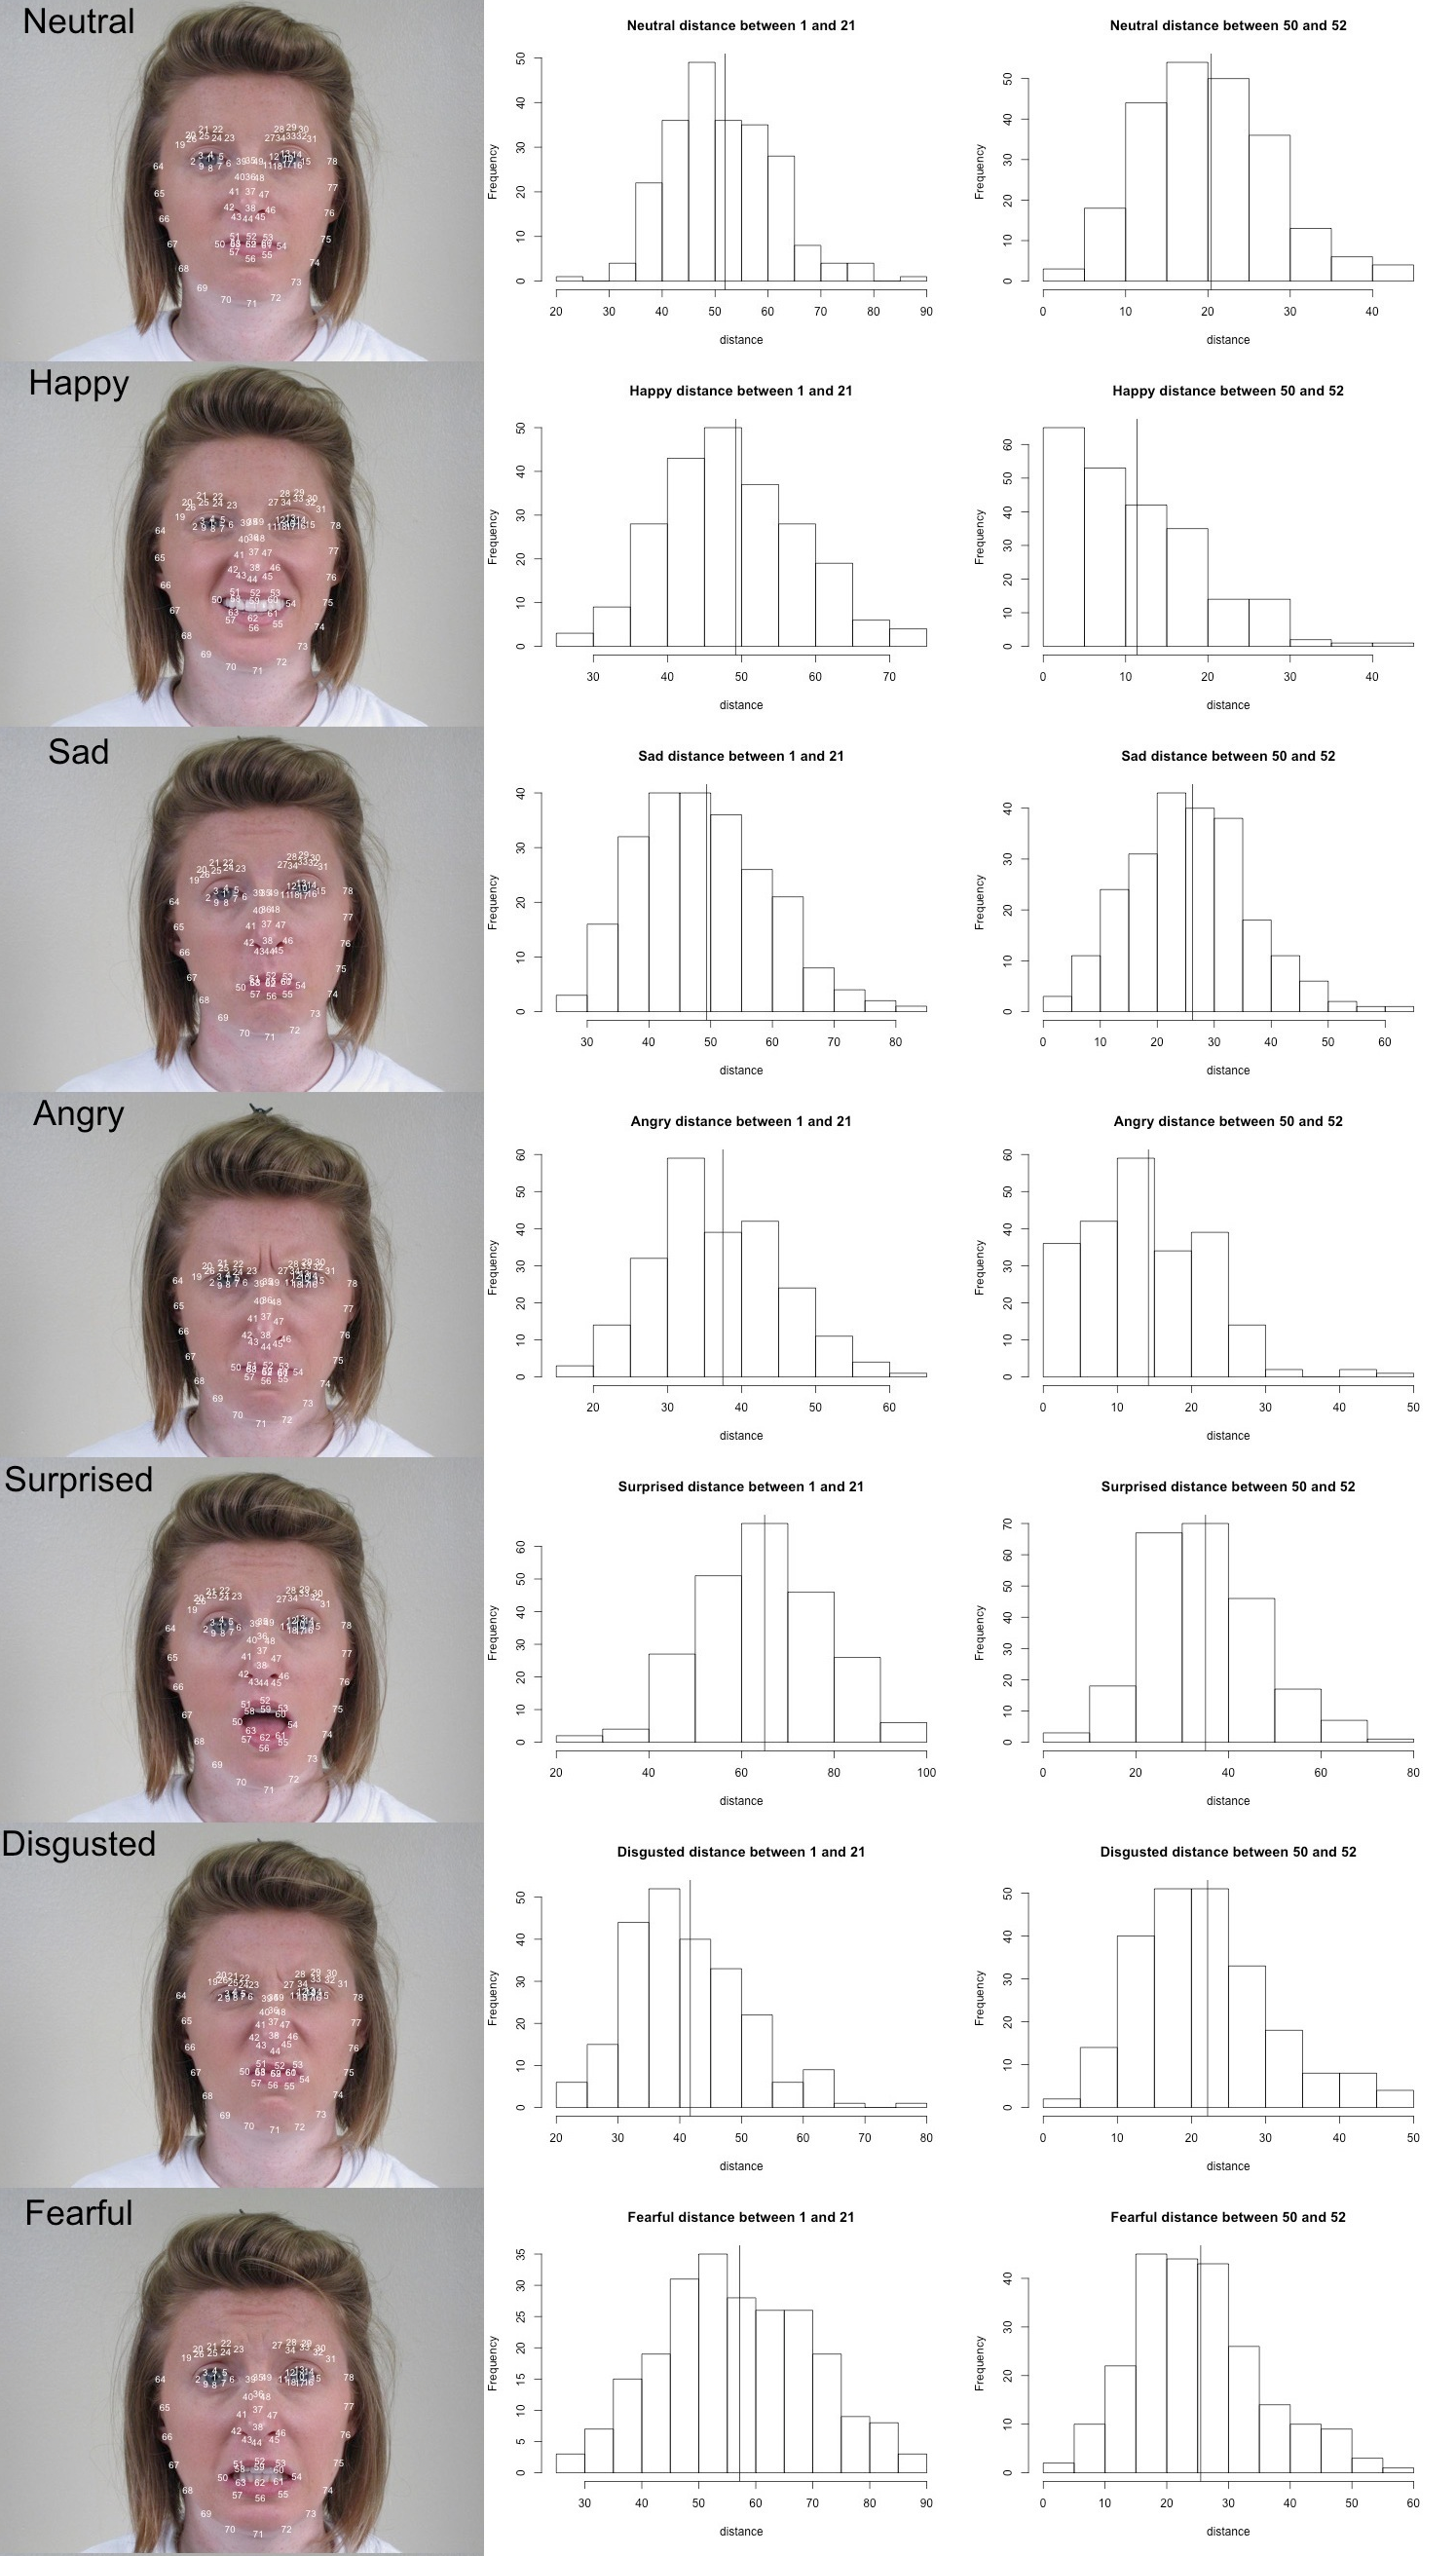
\includegraphics{../figs/feature_visualization.jpg}
\caption{Figure1}
\end{figure}

\texttt{feature.R} should be the wrapper for all your feature
engineering functions and options. The function \texttt{feature(\ )}
should have options that correspond to different scenarios for your
project and produces an R object that contains features and responses
that are required by all the models you are going to evaluate later.

\begin{itemize}
\tightlist
\item
  \texttt{feature.R}
\item
  Input: list of images or fiducial point
\item
  Output: an RData file that contains extracted features and
  corresponding responses
\end{itemize}

\begin{Shaded}
\begin{Highlighting}[]
\KeywordTok{source}\NormalTok{(}\StringTok{"../lib/feature.R"}\NormalTok{)}
\NormalTok{tm_feature_train <-}\StringTok{ }\OtherTok{NA}
\ControlFlowTok{if}\NormalTok{(run.feature.train)\{}
\NormalTok{  tm_feature_train <-}\StringTok{ }\KeywordTok{system.time}\NormalTok{(dat_train <-}\StringTok{ }\KeywordTok{feature}\NormalTok{(fiducial_pt_list, train_idx))}
  \KeywordTok{save}\NormalTok{(dat_train, tm_feature_train, }\DataTypeTok{file=}\StringTok{"../output/feature_train.RData"}\NormalTok{)}
\NormalTok{\}}\ControlFlowTok{else}\NormalTok{\{}
  \KeywordTok{load}\NormalTok{(}\DataTypeTok{file=}\StringTok{"../output/feature_train.RData"}\NormalTok{)}
\NormalTok{\}}

\NormalTok{tm_feature_test <-}\StringTok{ }\OtherTok{NA}
\ControlFlowTok{if}\NormalTok{(run.feature.test)\{}
\NormalTok{  tm_feature_test <-}\StringTok{ }\KeywordTok{system.time}\NormalTok{(dat_test <-}\StringTok{ }\KeywordTok{feature}\NormalTok{(fiducial_pt_list, test_idx))}
  \KeywordTok{save}\NormalTok{(dat_test, tm_feature_test, }\DataTypeTok{file=}\StringTok{"../output/feature_test.RData"}\NormalTok{)}
\NormalTok{\}}\ControlFlowTok{else}\NormalTok{\{}
  \KeywordTok{load}\NormalTok{(}\DataTypeTok{file=}\StringTok{"../output/feature_test.RData"}\NormalTok{)}
\NormalTok{\}}
\end{Highlighting}
\end{Shaded}

\newpage

\hypertarget{gradient-boosted-trees-gbm-model-baseline-model}{%
\subsection{Gradient Boosted Trees (gbm model) (Baseline
Model)}\label{gradient-boosted-trees-gbm-model-baseline-model}}

\hypertarget{step-4-train-a-classification-model-with-training-features-and-responses}{%
\subsubsection{Step 4: Train a classification model with training
features and
responses}\label{step-4-train-a-classification-model-with-training-features-and-responses}}

Call the train\_gbm model and test\_gbm model from library.

\texttt{train\_gbm.R} and \texttt{test\_gbm.R} should be wrappers for
all your model training steps and your classification/prediction steps.

\begin{itemize}
\tightlist
\item
  \texttt{train\_gbm.R}

  \begin{itemize}
  \tightlist
  \item
    Input: a data frame containing features and labels and a parameter
    list.
  \item
    Output:a trained model
  \end{itemize}
\item
  \texttt{test\_gbm.R}

  \begin{itemize}
  \tightlist
  \item
    Input: the fitted classification model using training data and
    processed features from testing images
  \item
    Input: an R object that contains a trained classifier.
  \item
    Output: training model specification
  \end{itemize}
\end{itemize}

\begin{Shaded}
\begin{Highlighting}[]
\KeywordTok{source}\NormalTok{(}\StringTok{"../lib/train_gbm.R"}\NormalTok{) }
\KeywordTok{source}\NormalTok{(}\StringTok{"../lib/test_gbm.R"}\NormalTok{)}
\KeywordTok{source}\NormalTok{(}\StringTok{"../lib/cross_validation_gbm.R"}\NormalTok{)}
\end{Highlighting}
\end{Shaded}

\hypertarget{model-selection-with-cross-validation}{%
\paragraph{Model selection with
cross-validation}\label{model-selection-with-cross-validation}}

\begin{itemize}
\tightlist
\item
  Do model selection by choosing among different values of training
  model parameters.
\end{itemize}

\begin{Shaded}
\begin{Highlighting}[]
\NormalTok{feature_train =}\StringTok{ }\KeywordTok{as.matrix}\NormalTok{(dat_train[, }\DecValTok{-6007}\NormalTok{])}
\NormalTok{label_train =}\StringTok{ }\KeywordTok{as.integer}\NormalTok{(dat_train}\OperatorTok{$}\NormalTok{label) }

\ControlFlowTok{if}\NormalTok{(run.cv.gbm)\{}
\NormalTok{  res_cv <-}\StringTok{ }\KeywordTok{matrix}\NormalTok{(}\DecValTok{0}\NormalTok{, }\DataTypeTok{nrow =} \KeywordTok{nrow}\NormalTok{(hyper_grid_gbm), }\DataTypeTok{ncol =} \DecValTok{4}\NormalTok{)}
  \ControlFlowTok{for}\NormalTok{(i }\ControlFlowTok{in} \DecValTok{1}\OperatorTok{:}\KeywordTok{nrow}\NormalTok{(hyper_grid_gbm))\{}
    \KeywordTok{cat}\NormalTok{(}\StringTok{"n.trees = "}\NormalTok{, hyper_grid_gbm}\OperatorTok{$}\NormalTok{n.trees[i], }\StringTok{", }
\StringTok{        shrinkage = "}\NormalTok{, hyper_grid_gbm}\OperatorTok{$}\NormalTok{shrinkage[i],}\StringTok{"}\CharTok{\textbackslash{}n}\StringTok{"}\NormalTok{, }\DataTypeTok{sep =} \StringTok{""}\NormalTok{)}
\NormalTok{    res_cv[i,] <-}\StringTok{ }\KeywordTok{cv.function}\NormalTok{(}\DataTypeTok{features =}\NormalTok{ feature_train, }\DataTypeTok{labels =}\NormalTok{ label_train,}
                              \DataTypeTok{num_trees =}\NormalTok{ hyper_grid_gbm}\OperatorTok{$}\NormalTok{n.trees[i], }
                              \DataTypeTok{shrink =}\NormalTok{ hyper_grid_gbm}\OperatorTok{$}\NormalTok{shrinkage[i], }
\NormalTok{                              K, }\DataTypeTok{reweight =}\NormalTok{ sample.reweight)}
  \KeywordTok{save}\NormalTok{(res_cv, }\DataTypeTok{file=}\StringTok{"../output/res_cv_gbm.RData"}\NormalTok{)}
\NormalTok{  \}}
\NormalTok{\}}\ControlFlowTok{else}\NormalTok{\{}
  \KeywordTok{load}\NormalTok{(}\StringTok{"../output/res_cv_gbm.RData"}\NormalTok{)}
\NormalTok{\}}
\end{Highlighting}
\end{Shaded}

*Visualize cross-validation results.

\begin{Shaded}
\begin{Highlighting}[]
\NormalTok{res_cv_gbm <-}\StringTok{ }\KeywordTok{as.data.frame}\NormalTok{(res_cv) }
\KeywordTok{colnames}\NormalTok{(res_cv_gbm) <-}\StringTok{ }\KeywordTok{c}\NormalTok{(}\StringTok{"mean_error"}\NormalTok{, }\StringTok{"sd_error"}\NormalTok{, }\StringTok{"mean_AUC"}\NormalTok{, }\StringTok{"sd_AUC"}\NormalTok{)}

\NormalTok{gbm_cv_results =}\StringTok{ }\KeywordTok{data.frame}\NormalTok{(hyper_grid_gbm, res_cv_gbm)}

\CommentTok{# a subset of cross-validated gbm models (15 total)}
\CommentTok{# see appendix for full table}
\NormalTok{gbm_cv_results[gbm_cv_results}\OperatorTok{$}\NormalTok{n.trees }\OperatorTok{==}\StringTok{ }\DecValTok{1200}\NormalTok{, ]}
\end{Highlighting}
\end{Shaded}

\begin{verbatim}
##    shrinkage n.trees mean_error   sd_error  mean_AUC     sd_AUC
## 6      0.001    1200  0.3494367 0.02250350 0.7269749 0.01997114
## 7      0.005    1200  0.3031100 0.01204216 0.7724047 0.01536358
## 8      0.010    1200  0.2905285 0.02278000 0.7885403 0.01576348
## 9      0.050    1200  0.2861576 0.02604993 0.8022183 0.01872366
## 10     0.100    1200  0.3004216 0.03110003 0.7986702 0.02425370
\end{verbatim}

\begin{Shaded}
\begin{Highlighting}[]
\CommentTok{# Mean Error}
\KeywordTok{ggplot}\NormalTok{(gbm_cv_results, }\KeywordTok{aes}\NormalTok{(}\KeywordTok{as.factor}\NormalTok{(shrinkage), }\KeywordTok{as.factor}\NormalTok{(n.trees), }\DataTypeTok{fill =}\NormalTok{ mean_error)) }\OperatorTok{+}\StringTok{ }
\StringTok{  }\KeywordTok{geom_tile}\NormalTok{()}
\end{Highlighting}
\end{Shaded}

\includegraphics{main_edited_files/figure-latex/cv_vis_gbm-1.pdf}

\begin{Shaded}
\begin{Highlighting}[]
\CommentTok{# Mean AUC}
\KeywordTok{ggplot}\NormalTok{(gbm_cv_results, }\KeywordTok{aes}\NormalTok{(}\KeywordTok{as.factor}\NormalTok{(shrinkage), }\KeywordTok{as.factor}\NormalTok{(n.trees), }\DataTypeTok{fill =}\NormalTok{ mean_AUC)) }\OperatorTok{+}\StringTok{ }
\StringTok{  }\KeywordTok{geom_tile}\NormalTok{()}
\end{Highlighting}
\end{Shaded}

\includegraphics{main_edited_files/figure-latex/cv_vis_gbm-2.pdf}

\begin{Shaded}
\begin{Highlighting}[]
\CommentTok{# Mean Error}
\CommentTok{# N.Trees = 600}
\KeywordTok{ggplot}\NormalTok{(gbm_cv_results[gbm_cv_results}\OperatorTok{$}\NormalTok{n.trees }\OperatorTok{==}\StringTok{ }\DecValTok{600}\NormalTok{, ],}
       \KeywordTok{aes}\NormalTok{(}\DataTypeTok{x =} \KeywordTok{as.factor}\NormalTok{(shrinkage), }\DataTypeTok{y =}\NormalTok{ mean_error, }
           \DataTypeTok{ymin =}\NormalTok{ mean_error }\OperatorTok{-}\StringTok{ }\NormalTok{sd_error, }\DataTypeTok{ymax =}\NormalTok{ mean_error }\OperatorTok{+}\StringTok{ }\NormalTok{sd_error)) }\OperatorTok{+}\StringTok{ }
\StringTok{    }\KeywordTok{geom_crossbar}\NormalTok{() }\OperatorTok{+}\StringTok{ }\KeywordTok{theme}\NormalTok{(}\DataTypeTok{axis.text.x =} \KeywordTok{element_text}\NormalTok{(}\DataTypeTok{angle =} \DecValTok{90}\NormalTok{, }\DataTypeTok{hjust =} \DecValTok{1}\NormalTok{))}
\end{Highlighting}
\end{Shaded}

\includegraphics{main_edited_files/figure-latex/cv_vis_gbm-3.pdf}

\begin{Shaded}
\begin{Highlighting}[]
\CommentTok{# N.Trees = 1200}
\KeywordTok{ggplot}\NormalTok{(gbm_cv_results[gbm_cv_results}\OperatorTok{$}\NormalTok{n.trees }\OperatorTok{==}\StringTok{ }\DecValTok{1200}\NormalTok{, ],}
       \KeywordTok{aes}\NormalTok{(}\DataTypeTok{x =} \KeywordTok{as.factor}\NormalTok{(shrinkage), }\DataTypeTok{y =}\NormalTok{ mean_error, }
           \DataTypeTok{ymin =}\NormalTok{ mean_error }\OperatorTok{-}\StringTok{ }\NormalTok{sd_error, }\DataTypeTok{ymax =}\NormalTok{ mean_error }\OperatorTok{+}\StringTok{ }\NormalTok{sd_error)) }\OperatorTok{+}\StringTok{ }
\StringTok{    }\KeywordTok{geom_crossbar}\NormalTok{() }\OperatorTok{+}\StringTok{ }\KeywordTok{theme}\NormalTok{(}\DataTypeTok{axis.text.x =} \KeywordTok{element_text}\NormalTok{(}\DataTypeTok{angle =} \DecValTok{90}\NormalTok{, }\DataTypeTok{hjust =} \DecValTok{1}\NormalTok{))}
\end{Highlighting}
\end{Shaded}

\includegraphics{main_edited_files/figure-latex/cv_vis_gbm-4.pdf}

\begin{Shaded}
\begin{Highlighting}[]
\CommentTok{# N.Trees = 1800}
\KeywordTok{ggplot}\NormalTok{(gbm_cv_results[gbm_cv_results}\OperatorTok{$}\NormalTok{n.trees }\OperatorTok{==}\StringTok{ }\DecValTok{1800}\NormalTok{, ],}
       \KeywordTok{aes}\NormalTok{(}\DataTypeTok{x =} \KeywordTok{as.factor}\NormalTok{(shrinkage), }\DataTypeTok{y =}\NormalTok{ mean_error, }
           \DataTypeTok{ymin =}\NormalTok{ mean_error }\OperatorTok{-}\StringTok{ }\NormalTok{sd_error, }\DataTypeTok{ymax =}\NormalTok{ mean_error }\OperatorTok{+}\StringTok{ }\NormalTok{sd_error)) }\OperatorTok{+}\StringTok{ }
\StringTok{    }\KeywordTok{geom_crossbar}\NormalTok{() }\OperatorTok{+}\StringTok{ }\KeywordTok{theme}\NormalTok{(}\DataTypeTok{axis.text.x =} \KeywordTok{element_text}\NormalTok{(}\DataTypeTok{angle =} \DecValTok{90}\NormalTok{, }\DataTypeTok{hjust =} \DecValTok{1}\NormalTok{))}
\end{Highlighting}
\end{Shaded}

\includegraphics{main_edited_files/figure-latex/cv_vis_gbm-5.pdf}

\begin{Shaded}
\begin{Highlighting}[]
\CommentTok{# Mean AUC}
\CommentTok{# N.Trees = 600}
\KeywordTok{ggplot}\NormalTok{(gbm_cv_results[gbm_cv_results}\OperatorTok{$}\NormalTok{n.trees }\OperatorTok{==}\StringTok{ }\DecValTok{600}\NormalTok{, ],}
       \KeywordTok{aes}\NormalTok{(}\DataTypeTok{x =} \KeywordTok{as.factor}\NormalTok{(shrinkage), }\DataTypeTok{y =}\NormalTok{ mean_AUC, }
           \DataTypeTok{ymin =}\NormalTok{ mean_AUC }\OperatorTok{-}\StringTok{ }\NormalTok{sd_AUC, }\DataTypeTok{ymax =}\NormalTok{ mean_AUC }\OperatorTok{+}\StringTok{ }\NormalTok{sd_AUC)) }\OperatorTok{+}\StringTok{ }
\StringTok{    }\KeywordTok{geom_crossbar}\NormalTok{() }\OperatorTok{+}\StringTok{ }\KeywordTok{theme}\NormalTok{(}\DataTypeTok{axis.text.x =} \KeywordTok{element_text}\NormalTok{(}\DataTypeTok{angle =} \DecValTok{90}\NormalTok{, }\DataTypeTok{hjust =} \DecValTok{1}\NormalTok{))}
\end{Highlighting}
\end{Shaded}

\includegraphics{main_edited_files/figure-latex/cv_vis_gbm-6.pdf}

\begin{Shaded}
\begin{Highlighting}[]
\CommentTok{# N.Trees = 1200}
\KeywordTok{ggplot}\NormalTok{(gbm_cv_results[gbm_cv_results}\OperatorTok{$}\NormalTok{n.trees }\OperatorTok{==}\StringTok{ }\DecValTok{1200}\NormalTok{, ],}
       \KeywordTok{aes}\NormalTok{(}\DataTypeTok{x =} \KeywordTok{as.factor}\NormalTok{(shrinkage), }\DataTypeTok{y =}\NormalTok{ mean_AUC, }
           \DataTypeTok{ymin =}\NormalTok{ mean_AUC }\OperatorTok{-}\StringTok{ }\NormalTok{sd_AUC, }\DataTypeTok{ymax =}\NormalTok{ mean_AUC }\OperatorTok{+}\StringTok{ }\NormalTok{sd_AUC)) }\OperatorTok{+}\StringTok{ }
\StringTok{    }\KeywordTok{geom_crossbar}\NormalTok{() }\OperatorTok{+}\StringTok{ }\KeywordTok{theme}\NormalTok{(}\DataTypeTok{axis.text.x =} \KeywordTok{element_text}\NormalTok{(}\DataTypeTok{angle =} \DecValTok{90}\NormalTok{, }\DataTypeTok{hjust =} \DecValTok{1}\NormalTok{))}
\end{Highlighting}
\end{Shaded}

\includegraphics{main_edited_files/figure-latex/cv_vis_gbm-7.pdf}

\begin{Shaded}
\begin{Highlighting}[]
\CommentTok{# N.Trees = 1800}
\KeywordTok{ggplot}\NormalTok{(gbm_cv_results[gbm_cv_results}\OperatorTok{$}\NormalTok{n.trees }\OperatorTok{==}\StringTok{ }\DecValTok{1800}\NormalTok{, ],}
       \KeywordTok{aes}\NormalTok{(}\DataTypeTok{x =} \KeywordTok{as.factor}\NormalTok{(shrinkage), }\DataTypeTok{y =}\NormalTok{ mean_AUC, }
           \DataTypeTok{ymin =}\NormalTok{ mean_AUC }\OperatorTok{-}\StringTok{ }\NormalTok{sd_AUC, }\DataTypeTok{ymax =}\NormalTok{ mean_AUC }\OperatorTok{+}\StringTok{ }\NormalTok{sd_AUC)) }\OperatorTok{+}\StringTok{ }
\StringTok{    }\KeywordTok{geom_crossbar}\NormalTok{() }\OperatorTok{+}\StringTok{ }\KeywordTok{theme}\NormalTok{(}\DataTypeTok{axis.text.x =} \KeywordTok{element_text}\NormalTok{(}\DataTypeTok{angle =} \DecValTok{90}\NormalTok{, }\DataTypeTok{hjust =} \DecValTok{1}\NormalTok{))}
\end{Highlighting}
\end{Shaded}

\includegraphics{main_edited_files/figure-latex/cv_vis_gbm-8.pdf}

\begin{itemize}
\tightlist
\item
  Choose the ``best'' parameter value
\end{itemize}

\begin{Shaded}
\begin{Highlighting}[]
\NormalTok{par_best_gbm_ind <-}\StringTok{ }\KeywordTok{which}\NormalTok{(gbm_cv_results}\OperatorTok{$}\NormalTok{mean_AUC }\OperatorTok{==}\StringTok{ }\KeywordTok{max}\NormalTok{(gbm_cv_results}\OperatorTok{$}\NormalTok{mean_AUC))}
\NormalTok{par_best_gbm_shrinkage <-}\StringTok{ }\NormalTok{gbm_cv_results}\OperatorTok{$}\NormalTok{shrinkage[par_best_gbm_ind]}
\NormalTok{par_best_gbm_n.trees <-}\StringTok{ }\NormalTok{gbm_cv_results}\OperatorTok{$}\NormalTok{n.trees[par_best_gbm_ind]}
\end{Highlighting}
\end{Shaded}

\begin{itemize}
\tightlist
\item
  Train the model with the entire training set using the selected model
  (model parameter) via cross-validation.
\end{itemize}

\begin{Shaded}
\begin{Highlighting}[]
\ControlFlowTok{if}\NormalTok{ (run.train.gbm) \{}
  \CommentTok{# training weights}
\NormalTok{  weight_train <-}\StringTok{ }\KeywordTok{rep}\NormalTok{(}\OtherTok{NA}\NormalTok{, }\KeywordTok{length}\NormalTok{(label_train))}
  \ControlFlowTok{for}\NormalTok{ (v }\ControlFlowTok{in} \KeywordTok{unique}\NormalTok{(label_train))\{}
\NormalTok{    weight_train[label_train }\OperatorTok{==}\StringTok{ }\NormalTok{v] =}\StringTok{ }\FloatTok{0.5} \OperatorTok{*}\StringTok{ }\KeywordTok{length}\NormalTok{(label_train) }\OperatorTok{/}\StringTok{ }\KeywordTok{length}\NormalTok{(label_train[label_train }\OperatorTok{==}\StringTok{ }\NormalTok{v])}
\NormalTok{  \}}
  
  \ControlFlowTok{if}\NormalTok{ (sample.reweight)\{}
\NormalTok{    tm_train_gbm <-}\StringTok{ }\KeywordTok{system.time}\NormalTok{(fit_train_gbm <-}\StringTok{ }\KeywordTok{train}\NormalTok{(feature_train, label_train, }\DataTypeTok{w =}\NormalTok{ weight_train, }
                                                       \DataTypeTok{num_trees =}\NormalTok{ par_best_gbm_n.trees, }
                                                       \DataTypeTok{shrink =}\NormalTok{ par_best_gbm_shrinkage))}
\NormalTok{  \} }\ControlFlowTok{else}\NormalTok{ \{}
\NormalTok{    tm_train_gbm <-}\StringTok{ }\KeywordTok{system.time}\NormalTok{(fit_train_gbm <-}\StringTok{ }\KeywordTok{train}\NormalTok{(feature_train, label_train, }\DataTypeTok{w =} \OtherTok{NULL}\NormalTok{, }
                                                       \DataTypeTok{num_trees =}\NormalTok{ par_best_gbm_n.trees,}
                                                       \DataTypeTok{shrink =}\NormalTok{ par_best_gbm_shrinkage))}
\NormalTok{  \}}
  \KeywordTok{save}\NormalTok{(fit_train_gbm, tm_train_gbm, }\DataTypeTok{file=}\StringTok{"../output/fit_train_gbm.RData"}\NormalTok{)}
  
\NormalTok{\} }\ControlFlowTok{else}\NormalTok{ \{}
  \KeywordTok{load}\NormalTok{(}\DataTypeTok{file=}\StringTok{"../output/fit_train_gbm.RData"}\NormalTok{)}
\NormalTok{\}}
\end{Highlighting}
\end{Shaded}

\hypertarget{step-5-run-test-on-test-images}{%
\subsubsection{Step 5: Run test on test
images}\label{step-5-run-test-on-test-images}}

\begin{Shaded}
\begin{Highlighting}[]
\NormalTok{feature_test <-}\StringTok{ }\KeywordTok{as.matrix}\NormalTok{(dat_test[, }\DecValTok{-6007}\NormalTok{])}
\NormalTok{label_test <-}\StringTok{ }\KeywordTok{as.integer}\NormalTok{(dat_test}\OperatorTok{$}\NormalTok{label)}

\NormalTok{tm_test_gbm =}\StringTok{ }\OtherTok{NA}

\ControlFlowTok{if}\NormalTok{(run.test.gbm)\{}
  \KeywordTok{load}\NormalTok{(}\DataTypeTok{file=}\StringTok{"../output/fit_train_gbm.RData"}\NormalTok{)}
\NormalTok{  tm_test_gbm <-}\StringTok{ }\KeywordTok{system.time}\NormalTok{(\{prob_pred <-}\StringTok{ }\KeywordTok{test}\NormalTok{(fit_train_gbm, feature_test, }\DataTypeTok{pred.type =} \StringTok{'response'}\NormalTok{); }
\NormalTok{                              label_pred <-}\StringTok{ }\KeywordTok{ifelse}\NormalTok{(prob_pred }\OperatorTok{>=}\StringTok{ }\FloatTok{0.5}\NormalTok{, }\DecValTok{1}\NormalTok{, }\DecValTok{0}\NormalTok{)\})}
\NormalTok{\}}
\end{Highlighting}
\end{Shaded}

\begin{itemize}
\tightlist
\item
  Evaluation
\end{itemize}

\begin{Shaded}
\begin{Highlighting}[]
\CommentTok{## reweight the test data to represent a balanced label distribution}

\NormalTok{weight_test <-}\StringTok{ }\KeywordTok{rep}\NormalTok{(}\OtherTok{NA}\NormalTok{, }\KeywordTok{length}\NormalTok{(label_test))}
\ControlFlowTok{for}\NormalTok{ (v }\ControlFlowTok{in} \KeywordTok{unique}\NormalTok{(label_test))\{}
\NormalTok{  weight_test[label_test }\OperatorTok{==}\StringTok{ }\NormalTok{v] =}\StringTok{ }\FloatTok{0.5} \OperatorTok{*}\StringTok{ }\KeywordTok{length}\NormalTok{(label_test) }\OperatorTok{/}\StringTok{ }\KeywordTok{length}\NormalTok{(label_test[label_test }\OperatorTok{==}\StringTok{ }\NormalTok{v])}
\NormalTok{\}}


\CommentTok{# convert the original 1-2 class into numeric 0s and 1s}
\NormalTok{label_test <-}\StringTok{ }\KeywordTok{ifelse}\NormalTok{(label_test }\OperatorTok{==}\StringTok{ }\DecValTok{2}\NormalTok{, }\DecValTok{0}\NormalTok{, }\DecValTok{1}\NormalTok{)}

\NormalTok{accu <-}\StringTok{ }\KeywordTok{sum}\NormalTok{(weight_test }\OperatorTok{*}\StringTok{ }\NormalTok{(label_pred }\OperatorTok{==}\StringTok{ }\NormalTok{label_test)) }\OperatorTok{/}\StringTok{ }\KeywordTok{sum}\NormalTok{(weight_test)}
\NormalTok{tpr.fpr <-}\StringTok{ }\KeywordTok{WeightedROC}\NormalTok{(prob_pred, label_test, weight_test)}
\NormalTok{auc <-}\StringTok{ }\KeywordTok{WeightedAUC}\NormalTok{(tpr.fpr)}
\end{Highlighting}
\end{Shaded}

\begin{verbatim}
## The accuracy of the gbm model (shinkage = 0.05, n.trees = 1200) is 74.4%.
\end{verbatim}

\begin{verbatim}
## The AUC of the gbm model (shinkage = 0.05, n.trees = 1200) is 0.8086568.
\end{verbatim}

\hypertarget{summarize-running-time}{%
\paragraph{Summarize Running Time}\label{summarize-running-time}}

Prediction performance matters, so does the running times for
constructing features and for training the model, especially when the
computation resource is limited.

\begin{verbatim}
## Time for constructing training features = 2.14 seconds
\end{verbatim}

\begin{verbatim}
## Time for constructing testing features = 0.16 seconds
\end{verbatim}

\begin{verbatim}
## Time for training gbm model = 233.97 seconds
\end{verbatim}

\begin{verbatim}
## Time for testing gbm model = 14.51 seconds
\end{verbatim}

\newpage

\hypertarget{xgboost-model-proposed-model}{%
\subsection{xgboost Model (Proposed
Model)}\label{xgboost-model-proposed-model}}

\hypertarget{step-4-train-a-classification-model-with-training-features-and-responses-1}{%
\subsubsection{Step 4: Train a classification model with training
features and
responses}\label{step-4-train-a-classification-model-with-training-features-and-responses-1}}

Call the train model and test model from library.

\texttt{train.R} and \texttt{test.R} should be wrappers for all your
model training steps and your classification/prediction steps.

\begin{itemize}
\tightlist
\item
  \texttt{train.R}

  \begin{itemize}
  \tightlist
  \item
    Input: a data frame containing features and labels and a parameter
    list.
  \item
    Output:a trained model
  \end{itemize}
\item
  \texttt{test.R}

  \begin{itemize}
  \tightlist
  \item
    Input: the fitted classification model using training data and
    processed features from testing images
  \item
    Input: an R object that contains a trained classifier.
  \item
    Output: training model specification
  \end{itemize}
\end{itemize}

\begin{Shaded}
\begin{Highlighting}[]
\KeywordTok{source}\NormalTok{(}\StringTok{"../lib/train_xgboost.R"}\NormalTok{) }
\KeywordTok{source}\NormalTok{(}\StringTok{"../lib/test_xgboost.R"}\NormalTok{) }
\KeywordTok{source}\NormalTok{(}\StringTok{"../lib/cross_validation_xgboost.R"}\NormalTok{) }
\end{Highlighting}
\end{Shaded}

\hypertarget{model-selection-with-cross-validation-1}{%
\paragraph{Model selection with
cross-validation}\label{model-selection-with-cross-validation-1}}

\begin{itemize}
\tightlist
\item
  Do model selection by choosing among different values of training
  model parameters.
\end{itemize}

\begin{Shaded}
\begin{Highlighting}[]
\NormalTok{feature_train =}\StringTok{ }\KeywordTok{as.matrix}\NormalTok{(dat_train[, }\DecValTok{-6007}\NormalTok{])}
\NormalTok{label_train =}\StringTok{ }\KeywordTok{as.integer}\NormalTok{(dat_train}\OperatorTok{$}\NormalTok{label) }

\ControlFlowTok{if}\NormalTok{(run.cv.xgboost)\{}
\NormalTok{  res_cv <-}\StringTok{ }\KeywordTok{matrix}\NormalTok{(}\DecValTok{0}\NormalTok{, }\DataTypeTok{nrow =} \KeywordTok{nrow}\NormalTok{(hyper_grid_xgboost), }\DataTypeTok{ncol =} \DecValTok{4}\NormalTok{)}
  \ControlFlowTok{for}\NormalTok{ (i }\ControlFlowTok{in} \DecValTok{1}\OperatorTok{:}\KeywordTok{nrow}\NormalTok{(hyper_grid_xgboost))\{}
    \KeywordTok{print}\NormalTok{(i)}
\NormalTok{    res_cv[i,] <-}\StringTok{ }\KeywordTok{cv.function}\NormalTok{(}\DataTypeTok{features =}\NormalTok{ feature_train, }\DataTypeTok{labels =}\NormalTok{ label_train,}
\NormalTok{                              K,}
                              \DataTypeTok{eta_val =}\NormalTok{ hyper_grid_xgboost}\OperatorTok{$}\NormalTok{eta[i], }
                              \DataTypeTok{lmd =}\NormalTok{ hyper_grid_xgboost}\OperatorTok{$}\NormalTok{lambda[i], }
                              \DataTypeTok{gam =}\NormalTok{ hyper_grid_xgboost}\OperatorTok{$}\NormalTok{gamma[i], }
                              \DataTypeTok{nr =}\NormalTok{ hyper_grid_xgboost}\OperatorTok{$}\NormalTok{nrounds[i])}
  \KeywordTok{save}\NormalTok{(res_cv, }\DataTypeTok{file=}\StringTok{"../output/res_cv_xgboost.RData"}\NormalTok{)}
\NormalTok{  \}}
\NormalTok{\}}\ControlFlowTok{else}\NormalTok{\{}
  \KeywordTok{load}\NormalTok{(}\StringTok{"../output/res_cv_xgboost.RData"}\NormalTok{)}
\NormalTok{\}}
\end{Highlighting}
\end{Shaded}

*Visualize cross-validation results.

\begin{Shaded}
\begin{Highlighting}[]
\NormalTok{res_cv_xgboost <-}\StringTok{ }\KeywordTok{as.data.frame}\NormalTok{(res_cv) }
\KeywordTok{colnames}\NormalTok{(res_cv_xgboost) <-}\StringTok{ }\KeywordTok{c}\NormalTok{(}\StringTok{"mean_error"}\NormalTok{, }\StringTok{"sd_error"}\NormalTok{, }\StringTok{"mean_AUC"}\NormalTok{, }\StringTok{"sd_AUC"}\NormalTok{)}

\NormalTok{res_cv_xgboost_cv_results =}\StringTok{ }\KeywordTok{data.frame}\NormalTok{(hyper_grid_xgboost, res_cv_xgboost)}

\CommentTok{# a subset of cross-validated xgboost models (150 total)}
\CommentTok{# see appendix for full table}
\NormalTok{res_cv_xgboost_cv_results[res_cv_xgboost_cv_results}\OperatorTok{$}\NormalTok{nrounds }\OperatorTok{==}\StringTok{ }\DecValTok{1200} \OperatorTok{&}\StringTok{ }\NormalTok{res_cv_xgboost_cv_results}\OperatorTok{$}\NormalTok{gamma }\OperatorTok{==}\StringTok{ }\DecValTok{0} \OperatorTok{&}\StringTok{ }\NormalTok{res_cv_xgboost_cv_results}\OperatorTok{$}\NormalTok{lambda }\OperatorTok{==}\StringTok{ }\FloatTok{0.05}\NormalTok{, ]}
\end{Highlighting}
\end{Shaded}

\begin{verbatim}
##     eta lambda gamma nrounds mean_error    sd_error  mean_AUC     sd_AUC
## 66 0.01   0.05     0    1200  0.4615955 0.009160897 0.7786848 0.01608024
## 67 0.05   0.05     0    1200  0.4054330 0.018383518 0.8083090 0.01479400
## 68 0.10   0.05     0    1200  0.3813304 0.022033539 0.8034491 0.02412093
## 69 0.20   0.05     0    1200  0.3574039 0.020227396 0.7956913 0.02202451
## 70 0.30   0.05     0    1200  0.3481230 0.011280241 0.7934894 0.02261126
\end{verbatim}

\begin{Shaded}
\begin{Highlighting}[]
\CommentTok{# Mean Error}
\KeywordTok{ggplot}\NormalTok{(res_cv_xgboost_cv_results, }\KeywordTok{aes}\NormalTok{(}\KeywordTok{as.factor}\NormalTok{(nrounds), }\KeywordTok{as.factor}\NormalTok{(eta), }\DataTypeTok{fill =}\NormalTok{ mean_error)) }\OperatorTok{+}\StringTok{ }
\StringTok{  }\KeywordTok{geom_tile}\NormalTok{()}
\end{Highlighting}
\end{Shaded}

\includegraphics{main_edited_files/figure-latex/cv_vis_xgboost-1.pdf}

\begin{Shaded}
\begin{Highlighting}[]
\CommentTok{# Mean AUC}
\KeywordTok{ggplot}\NormalTok{(res_cv_xgboost_cv_results, }\KeywordTok{aes}\NormalTok{(}\KeywordTok{as.factor}\NormalTok{(nrounds), }\KeywordTok{as.factor}\NormalTok{(eta), }\DataTypeTok{fill =}\NormalTok{ mean_AUC)) }\OperatorTok{+}\StringTok{ }
\StringTok{  }\KeywordTok{geom_tile}\NormalTok{()}
\end{Highlighting}
\end{Shaded}

\includegraphics{main_edited_files/figure-latex/cv_vis_xgboost-2.pdf}

\begin{Shaded}
\begin{Highlighting}[]
\CommentTok{# Mean Error}
\CommentTok{# nrounds = 600}
\KeywordTok{ggplot}\NormalTok{(res_cv_xgboost_cv_results[res_cv_xgboost_cv_results}\OperatorTok{$}\NormalTok{nrounds }\OperatorTok{==}\StringTok{ }\DecValTok{600} \OperatorTok{&}\StringTok{ }\NormalTok{res_cv_xgboost_cv_results}\OperatorTok{$}\NormalTok{gamma }\OperatorTok{==}\StringTok{ }\DecValTok{0} \OperatorTok{&}\StringTok{ }\NormalTok{res_cv_xgboost_cv_results}\OperatorTok{$}\NormalTok{lambda }\OperatorTok{==}\StringTok{ }\FloatTok{0.05}\NormalTok{, ],}
       \KeywordTok{aes}\NormalTok{(}\DataTypeTok{x =} \KeywordTok{as.factor}\NormalTok{(eta), }\DataTypeTok{y =}\NormalTok{ mean_error, }
           \DataTypeTok{ymin =}\NormalTok{ mean_error }\OperatorTok{-}\StringTok{ }\NormalTok{sd_error, }\DataTypeTok{ymax =}\NormalTok{ mean_error }\OperatorTok{+}\StringTok{ }\NormalTok{sd_error)) }\OperatorTok{+}\StringTok{ }
\StringTok{    }\KeywordTok{geom_crossbar}\NormalTok{() }\OperatorTok{+}\StringTok{ }\KeywordTok{theme}\NormalTok{(}\DataTypeTok{axis.text.x =} \KeywordTok{element_text}\NormalTok{(}\DataTypeTok{angle =} \DecValTok{90}\NormalTok{, }\DataTypeTok{hjust =} \DecValTok{1}\NormalTok{))}
\end{Highlighting}
\end{Shaded}

\includegraphics{main_edited_files/figure-latex/cv_vis_xgboost-3.pdf}

\begin{Shaded}
\begin{Highlighting}[]
\CommentTok{# nrounds = 1200}
\KeywordTok{ggplot}\NormalTok{(res_cv_xgboost_cv_results[res_cv_xgboost_cv_results}\OperatorTok{$}\NormalTok{nrounds }\OperatorTok{==}\StringTok{ }\DecValTok{1200} \OperatorTok{&}\StringTok{ }\NormalTok{res_cv_xgboost_cv_results}\OperatorTok{$}\NormalTok{gamma }\OperatorTok{==}\StringTok{ }\DecValTok{0} \OperatorTok{&}\StringTok{ }\NormalTok{res_cv_xgboost_cv_results}\OperatorTok{$}\NormalTok{lambda }\OperatorTok{==}\StringTok{ }\FloatTok{0.05}\NormalTok{, ],}
       \KeywordTok{aes}\NormalTok{(}\DataTypeTok{x =} \KeywordTok{as.factor}\NormalTok{(eta), }\DataTypeTok{y =}\NormalTok{ mean_error, }
           \DataTypeTok{ymin =}\NormalTok{ mean_error }\OperatorTok{-}\StringTok{ }\NormalTok{sd_error, }\DataTypeTok{ymax =}\NormalTok{ mean_error }\OperatorTok{+}\StringTok{ }\NormalTok{sd_error)) }\OperatorTok{+}\StringTok{ }
\StringTok{    }\KeywordTok{geom_crossbar}\NormalTok{() }\OperatorTok{+}\StringTok{ }\KeywordTok{theme}\NormalTok{(}\DataTypeTok{axis.text.x =} \KeywordTok{element_text}\NormalTok{(}\DataTypeTok{angle =} \DecValTok{90}\NormalTok{, }\DataTypeTok{hjust =} \DecValTok{1}\NormalTok{))}
\end{Highlighting}
\end{Shaded}

\includegraphics{main_edited_files/figure-latex/cv_vis_xgboost-4.pdf}

\begin{Shaded}
\begin{Highlighting}[]
\CommentTok{# nrounds = 1800}
\KeywordTok{ggplot}\NormalTok{(res_cv_xgboost_cv_results[res_cv_xgboost_cv_results}\OperatorTok{$}\NormalTok{nrounds }\OperatorTok{==}\StringTok{ }\DecValTok{1800} \OperatorTok{&}\StringTok{ }\NormalTok{res_cv_xgboost_cv_results}\OperatorTok{$}\NormalTok{gamma }\OperatorTok{==}\StringTok{ }\DecValTok{0} \OperatorTok{&}\StringTok{ }\NormalTok{res_cv_xgboost_cv_results}\OperatorTok{$}\NormalTok{lambda }\OperatorTok{==}\StringTok{ }\FloatTok{0.05}\NormalTok{, ],}
       \KeywordTok{aes}\NormalTok{(}\DataTypeTok{x =} \KeywordTok{as.factor}\NormalTok{(eta), }\DataTypeTok{y =}\NormalTok{ mean_error, }
           \DataTypeTok{ymin =}\NormalTok{ mean_error }\OperatorTok{-}\StringTok{ }\NormalTok{sd_error, }\DataTypeTok{ymax =}\NormalTok{ mean_error }\OperatorTok{+}\StringTok{ }\NormalTok{sd_error)) }\OperatorTok{+}\StringTok{ }
\StringTok{    }\KeywordTok{geom_crossbar}\NormalTok{() }\OperatorTok{+}\StringTok{ }\KeywordTok{theme}\NormalTok{(}\DataTypeTok{axis.text.x =} \KeywordTok{element_text}\NormalTok{(}\DataTypeTok{angle =} \DecValTok{90}\NormalTok{, }\DataTypeTok{hjust =} \DecValTok{1}\NormalTok{))}
\end{Highlighting}
\end{Shaded}

\includegraphics{main_edited_files/figure-latex/cv_vis_xgboost-5.pdf}

\begin{Shaded}
\begin{Highlighting}[]
\CommentTok{# Mean AUC}
\CommentTok{# nrounds = 600}
\KeywordTok{ggplot}\NormalTok{(res_cv_xgboost_cv_results[res_cv_xgboost_cv_results}\OperatorTok{$}\NormalTok{nrounds }\OperatorTok{==}\StringTok{ }\DecValTok{600} \OperatorTok{&}\StringTok{ }\NormalTok{res_cv_xgboost_cv_results}\OperatorTok{$}\NormalTok{gamma }\OperatorTok{==}\StringTok{ }\DecValTok{0} \OperatorTok{&}\StringTok{ }\NormalTok{res_cv_xgboost_cv_results}\OperatorTok{$}\NormalTok{lambda }\OperatorTok{==}\StringTok{ }\FloatTok{0.05}\NormalTok{, ],}
       \KeywordTok{aes}\NormalTok{(}\DataTypeTok{x =} \KeywordTok{as.factor}\NormalTok{(eta), }\DataTypeTok{y =}\NormalTok{ mean_AUC, }
           \DataTypeTok{ymin =}\NormalTok{ mean_AUC }\OperatorTok{-}\StringTok{ }\NormalTok{sd_AUC, }\DataTypeTok{ymax =}\NormalTok{ mean_AUC }\OperatorTok{+}\StringTok{ }\NormalTok{sd_AUC)) }\OperatorTok{+}\StringTok{ }
\StringTok{    }\KeywordTok{geom_crossbar}\NormalTok{() }\OperatorTok{+}\StringTok{ }\KeywordTok{theme}\NormalTok{(}\DataTypeTok{axis.text.x =} \KeywordTok{element_text}\NormalTok{(}\DataTypeTok{angle =} \DecValTok{90}\NormalTok{, }\DataTypeTok{hjust =} \DecValTok{1}\NormalTok{))}
\end{Highlighting}
\end{Shaded}

\includegraphics{main_edited_files/figure-latex/cv_vis_xgboost-6.pdf}

\begin{Shaded}
\begin{Highlighting}[]
\CommentTok{# nrounds = 1200}
\KeywordTok{ggplot}\NormalTok{(res_cv_xgboost_cv_results[res_cv_xgboost_cv_results}\OperatorTok{$}\NormalTok{nrounds }\OperatorTok{==}\StringTok{ }\DecValTok{1200} \OperatorTok{&}\StringTok{ }\NormalTok{res_cv_xgboost_cv_results}\OperatorTok{$}\NormalTok{gamma }\OperatorTok{==}\StringTok{ }\DecValTok{0} \OperatorTok{&}\StringTok{ }\NormalTok{res_cv_xgboost_cv_results}\OperatorTok{$}\NormalTok{lambda }\OperatorTok{==}\StringTok{ }\FloatTok{0.05}\NormalTok{, ],}
       \KeywordTok{aes}\NormalTok{(}\DataTypeTok{x =} \KeywordTok{as.factor}\NormalTok{(eta), }\DataTypeTok{y =}\NormalTok{ mean_AUC, }
           \DataTypeTok{ymin =}\NormalTok{ mean_AUC }\OperatorTok{-}\StringTok{ }\NormalTok{sd_AUC, }\DataTypeTok{ymax =}\NormalTok{ mean_AUC }\OperatorTok{+}\StringTok{ }\NormalTok{sd_AUC)) }\OperatorTok{+}\StringTok{ }
\StringTok{    }\KeywordTok{geom_crossbar}\NormalTok{() }\OperatorTok{+}\StringTok{ }\KeywordTok{theme}\NormalTok{(}\DataTypeTok{axis.text.x =} \KeywordTok{element_text}\NormalTok{(}\DataTypeTok{angle =} \DecValTok{90}\NormalTok{, }\DataTypeTok{hjust =} \DecValTok{1}\NormalTok{))}
\end{Highlighting}
\end{Shaded}

\includegraphics{main_edited_files/figure-latex/cv_vis_xgboost-7.pdf}

\begin{Shaded}
\begin{Highlighting}[]
\CommentTok{# nrounds = 1800}
\KeywordTok{ggplot}\NormalTok{(res_cv_xgboost_cv_results[res_cv_xgboost_cv_results}\OperatorTok{$}\NormalTok{nrounds }\OperatorTok{==}\StringTok{ }\DecValTok{1800} \OperatorTok{&}\StringTok{ }\NormalTok{res_cv_xgboost_cv_results}\OperatorTok{$}\NormalTok{gamma }\OperatorTok{==}\StringTok{ }\DecValTok{0} \OperatorTok{&}\StringTok{ }\NormalTok{res_cv_xgboost_cv_results}\OperatorTok{$}\NormalTok{lambda }\OperatorTok{==}\StringTok{ }\FloatTok{0.05}\NormalTok{, ],}
       \KeywordTok{aes}\NormalTok{(}\DataTypeTok{x =} \KeywordTok{as.factor}\NormalTok{(eta), }\DataTypeTok{y =}\NormalTok{ mean_AUC, }
           \DataTypeTok{ymin =}\NormalTok{ mean_AUC }\OperatorTok{-}\StringTok{ }\NormalTok{sd_AUC, }\DataTypeTok{ymax =}\NormalTok{ mean_AUC }\OperatorTok{+}\StringTok{ }\NormalTok{sd_AUC)) }\OperatorTok{+}\StringTok{ }
\StringTok{    }\KeywordTok{geom_crossbar}\NormalTok{() }\OperatorTok{+}\StringTok{ }\KeywordTok{theme}\NormalTok{(}\DataTypeTok{axis.text.x =} \KeywordTok{element_text}\NormalTok{(}\DataTypeTok{angle =} \DecValTok{90}\NormalTok{, }\DataTypeTok{hjust =} \DecValTok{1}\NormalTok{))}
\end{Highlighting}
\end{Shaded}

\includegraphics{main_edited_files/figure-latex/cv_vis_xgboost-8.pdf}

\begin{itemize}
\tightlist
\item
  Choose the ``best'' parameter value
\end{itemize}

\begin{Shaded}
\begin{Highlighting}[]
\NormalTok{par_best_res_cv_xgboost_cv_results_ind <-}\StringTok{ }
\StringTok{  }\KeywordTok{which}\NormalTok{(res_cv_xgboost_cv_results}\OperatorTok{$}\NormalTok{mean_AUC }\OperatorTok{==}\StringTok{ }\KeywordTok{max}\NormalTok{(res_cv_xgboost_cv_results}\OperatorTok{$}\NormalTok{mean_AUC))}

\NormalTok{par_best_res_cv_xgboost_cv_results_eta <-}\StringTok{ }\NormalTok{res_cv_xgboost_cv_results}\OperatorTok{$}\NormalTok{eta[par_best_res_cv_xgboost_cv_results_ind]}
\NormalTok{par_best_res_cv_xgboost_cv_results_lambda <-}\StringTok{ }\NormalTok{res_cv_xgboost_cv_results}\OperatorTok{$}\NormalTok{lambda[par_best_res_cv_xgboost_cv_results_ind]}
\NormalTok{par_best_res_cv_xgboost_cv_results_gamma <-}\StringTok{ }\NormalTok{res_cv_xgboost_cv_results}\OperatorTok{$}\NormalTok{gamma[par_best_res_cv_xgboost_cv_results_ind]}
\NormalTok{par_best_res_cv_xgboost_cv_results_nrounds <-}\StringTok{ }\NormalTok{res_cv_xgboost_cv_results}\OperatorTok{$}\NormalTok{nrounds[par_best_res_cv_xgboost_cv_results_ind]}
\end{Highlighting}
\end{Shaded}

\begin{itemize}
\tightlist
\item
  Train the model with the entire training set using the selected model
  (model parameter) via cross-validation.
\end{itemize}

\begin{Shaded}
\begin{Highlighting}[]
\ControlFlowTok{if}\NormalTok{ (run.train.xgboost) \{}
  \CommentTok{# training weights}
\NormalTok{  weight_train <-}\StringTok{ }\KeywordTok{rep}\NormalTok{(}\OtherTok{NA}\NormalTok{, }\KeywordTok{length}\NormalTok{(label_train))}
  \ControlFlowTok{for}\NormalTok{ (v }\ControlFlowTok{in} \KeywordTok{unique}\NormalTok{(label_train))\{}
\NormalTok{    weight_train[label_train }\OperatorTok{==}\StringTok{ }\NormalTok{v] =}\StringTok{ }\FloatTok{0.5} \OperatorTok{*}\StringTok{ }\KeywordTok{length}\NormalTok{(label_train) }\OperatorTok{/}\StringTok{ }\KeywordTok{length}\NormalTok{(label_train[label_train }\OperatorTok{==}\StringTok{ }\NormalTok{v])}
\NormalTok{  \}}

  \ControlFlowTok{if}\NormalTok{ (sample.reweight)\{}
\NormalTok{    tm_train_xgboost <-}\StringTok{ }\KeywordTok{system.time}\NormalTok{(fit_train_xgboost <-}\StringTok{ }\KeywordTok{train}\NormalTok{(}\DataTypeTok{features =}\NormalTok{ feature_train, }\DataTypeTok{labels =}\NormalTok{ label_train,}
                                                                 \DataTypeTok{w =}\NormalTok{  weight_train,}
                                                                 \DataTypeTok{eta_val =}\NormalTok{ par_best_res_cv_xgboost_cv_results_eta,}
                                                                 \DataTypeTok{lmd =}\NormalTok{ par_best_res_cv_xgboost_cv_results_lambda,}
                                                                 \DataTypeTok{gam =}\NormalTok{ par_best_res_cv_xgboost_cv_results_gamma,}
                                                                 \DataTypeTok{nr =}\NormalTok{ par_best_res_cv_xgboost_cv_results_nrounds))}

\NormalTok{  \} }\ControlFlowTok{else}\NormalTok{ \{}

\NormalTok{    tm_train_xgboost <-}\StringTok{ }\KeywordTok{system.time}\NormalTok{(fit_train_xgboost <-}\StringTok{ }\KeywordTok{train}\NormalTok{(}\DataTypeTok{features =}\NormalTok{ feature_train, }\DataTypeTok{labels =}\NormalTok{ label_train,}
                                                                 \DataTypeTok{w =}  \OtherTok{NULL}\NormalTok{, }
                                                                 \DataTypeTok{eta_val =}\NormalTok{ par_best_res_cv_xgboost_cv_results_eta, }
                                                                 \DataTypeTok{lmd =}\NormalTok{ par_best_res_cv_xgboost_cv_results_lambda,}
                                                                 \DataTypeTok{gam =}\NormalTok{ par_best_res_cv_xgboost_cv_results_gamma,}
                                                                 \DataTypeTok{nr =}\NormalTok{ par_best_res_cv_xgboost_cv_results_nrounds))}
\NormalTok{  \}}
  \KeywordTok{save}\NormalTok{(fit_train_xgboost, tm_train_xgboost, }\DataTypeTok{file=}\StringTok{"../output/fit_train_xgboost.RData"}\NormalTok{)}
  
\NormalTok{\} }\ControlFlowTok{else}\NormalTok{ \{}
  \KeywordTok{load}\NormalTok{(}\DataTypeTok{file=}\StringTok{"../output/fit_train_xgboost.RData"}\NormalTok{)}
\NormalTok{\}}
\end{Highlighting}
\end{Shaded}

\hypertarget{step-5-run-test-on-test-images-1}{%
\subsubsection{Step 5: Run test on test
images}\label{step-5-run-test-on-test-images-1}}

\begin{Shaded}
\begin{Highlighting}[]
\NormalTok{feature_test <-}\StringTok{ }\KeywordTok{as.matrix}\NormalTok{(dat_test[, }\DecValTok{-6007}\NormalTok{])}
\NormalTok{label_test <-}\StringTok{ }\KeywordTok{as.integer}\NormalTok{(dat_test}\OperatorTok{$}\NormalTok{label)}

\NormalTok{tm_test_xgboost=}\StringTok{ }\OtherTok{NA}

\ControlFlowTok{if}\NormalTok{(run.test.xgboost)\{}
  \KeywordTok{load}\NormalTok{(}\DataTypeTok{file=}\StringTok{"../output/fit_train_xgboost.RData"}\NormalTok{)}
\NormalTok{  tm_test_xgboost <-}\StringTok{ }\KeywordTok{system.time}\NormalTok{(\{prob_pred <-}\StringTok{ }\KeywordTok{predict}\NormalTok{(fit_train_xgboost, feature_test); }
\NormalTok{                              label_pred <-}\StringTok{ }\KeywordTok{ifelse}\NormalTok{(prob_pred }\OperatorTok{>=}\StringTok{ }\FloatTok{0.5}\NormalTok{, }\DecValTok{1}\NormalTok{, }\DecValTok{0}\NormalTok{)\})}
\NormalTok{\}}
\end{Highlighting}
\end{Shaded}

\begin{itemize}
\tightlist
\item
  Evaluation
\end{itemize}

\begin{Shaded}
\begin{Highlighting}[]
\CommentTok{## reweight the test data to represent a balanced label distribution}
\NormalTok{weight_test <-}\StringTok{ }\KeywordTok{rep}\NormalTok{(}\OtherTok{NA}\NormalTok{, }\KeywordTok{length}\NormalTok{(label_test))}
\ControlFlowTok{for}\NormalTok{ (v }\ControlFlowTok{in} \KeywordTok{unique}\NormalTok{(label_test))\{}
\NormalTok{  weight_test[label_test }\OperatorTok{==}\StringTok{ }\NormalTok{v] =}\StringTok{ }\FloatTok{0.5} \OperatorTok{*}\StringTok{ }\KeywordTok{length}\NormalTok{(label_test) }\OperatorTok{/}\StringTok{ }\KeywordTok{length}\NormalTok{(label_test[label_test }\OperatorTok{==}\StringTok{ }\NormalTok{v])}
\NormalTok{\}}

\CommentTok{# convert the original 1-2 class into numeric 0s and 1s}
\NormalTok{label_test <-}\StringTok{ }\KeywordTok{ifelse}\NormalTok{(label_test }\OperatorTok{==}\StringTok{ }\DecValTok{2}\NormalTok{, }\DecValTok{0}\NormalTok{, }\DecValTok{1}\NormalTok{)}

\NormalTok{accu <-}\StringTok{ }\KeywordTok{sum}\NormalTok{(weight_test }\OperatorTok{*}\StringTok{ }\NormalTok{(label_pred }\OperatorTok{==}\StringTok{ }\NormalTok{label_test)) }\OperatorTok{/}\StringTok{ }\KeywordTok{sum}\NormalTok{(weight_test)}
\NormalTok{tpr.fpr <-}\StringTok{ }\KeywordTok{WeightedROC}\NormalTok{(prob_pred, label_test, weight_test)}
\NormalTok{auc <-}\StringTok{ }\KeywordTok{WeightedAUC}\NormalTok{(tpr.fpr)}
\end{Highlighting}
\end{Shaded}

\begin{verbatim}
## The accuracy of the xgboost model (eta = 0.05, nrounds = 1200, lambda = 0.05, gamma = 0) is 70.35789%.
\end{verbatim}

\begin{verbatim}
## The AUC of the xgboost model (eta = 0.05, nrounds = 1200, lambda = 0.05, gamma = 0) is 0.7965979.
\end{verbatim}

\hypertarget{summarize-running-time-1}{%
\paragraph{Summarize Running Time}\label{summarize-running-time-1}}

Prediction performance matters, so does the running times for
constructing features and for training the model, especially when the
computation resource is limited.

\begin{verbatim}
## Time for training xgboost model = 148.91 seconds
\end{verbatim}

\begin{verbatim}
## Time for testing xgboost model = 0.07 seconds
\end{verbatim}

\newpage

\hypertarget{other-models}{%
\subsection{Other Models}\label{other-models}}

\hypertarget{principal-components-analysis-pca-support-vector-machines-svms}{%
\subsection{Principal Components Analysis (PCA) + Support Vector
Machines
(SVMs)}\label{principal-components-analysis-pca-support-vector-machines-svms}}

\hypertarget{step-4-train-a-classification-model-with-training-features-and-responses-2}{%
\subsubsection{Step 4: Train a classification model with training
features and
responses}\label{step-4-train-a-classification-model-with-training-features-and-responses-2}}

Call the train model and test model from library.

\texttt{train.R} and \texttt{test.R} should be wrappers for all your
model training steps and your classification/prediction steps.

\begin{itemize}
\tightlist
\item
  \texttt{train.R}

  \begin{itemize}
  \tightlist
  \item
    Input: a data frame containing features and labels and a parameter
    list.
  \item
    Output:a trained model
  \end{itemize}
\item
  \texttt{test.R}

  \begin{itemize}
  \tightlist
  \item
    Input: the fitted classification model using training data and
    processed features from testing images
  \item
    Input: an R object that contains a trained classifier.
  \item
    Output: training model specification
  \end{itemize}
\item
  In this Starter Code, we use logistic regression with LASSO penalty to
  do classification.
\end{itemize}

\hypertarget{model-selection-with-cross-validation-2}{%
\paragraph{Model selection with
cross-validation}\label{model-selection-with-cross-validation-2}}

\begin{itemize}
\tightlist
\item
  Do model selection by choosing among different values of training
  model parameters.
\end{itemize}

*Visualize cross-validation results.

\begin{itemize}
\item
  Choose the ``best'' parameter value
\item
  Train the model with the entire training set using the selected model
  (model parameter) via cross-validation.
\end{itemize}

\hypertarget{step-5-run-test-on-test-images-2}{%
\subsubsection{Step 5: Run test on test
images}\label{step-5-run-test-on-test-images-2}}

\begin{itemize}
\tightlist
\item
  Evaluation
\end{itemize}

\hypertarget{summarize-running-time-2}{%
\paragraph{Summarize Running Time}\label{summarize-running-time-2}}

Prediction performance matters, so does the running times for
constructing features and for training the model, especially when the
computation resource is limited.

\newpage

\hypertarget{random-forests}{%
\subsection{Random Forests}\label{random-forests}}

\hypertarget{step-4-train-a-classification-model-with-training-features-and-responses-3}{%
\subsubsection{Step 4: Train a classification model with training
features and
responses}\label{step-4-train-a-classification-model-with-training-features-and-responses-3}}

Call the train model and test model from library.

\texttt{train.R} and \texttt{test.R} should be wrappers for all your
model training steps and your classification/prediction steps.

\begin{itemize}
\tightlist
\item
  \texttt{train.R}

  \begin{itemize}
  \tightlist
  \item
    Input: a data frame containing features and labels and a parameter
    list.
  \item
    Output:a trained model
  \end{itemize}
\item
  \texttt{test.R}

  \begin{itemize}
  \tightlist
  \item
    Input: the fitted classification model using training data and
    processed features from testing images
  \item
    Input: an R object that contains a trained classifier.
  \item
    Output: training model specification
  \end{itemize}
\item
  In this Starter Code, we use logistic regression with LASSO penalty to
  do classification.
\end{itemize}

\begin{Shaded}
\begin{Highlighting}[]
\KeywordTok{library}\NormalTok{(magrittr)    }\CommentTok{#### NEED TO INSTALL THIS PACKAGE ON TO BUT ONLY IF WE STILL NEED IT}
\KeywordTok{source}\NormalTok{(}\StringTok{"../lib/train.R"}\NormalTok{) }
\KeywordTok{source}\NormalTok{(}\StringTok{"../lib/test.R"}\NormalTok{)}
\end{Highlighting}
\end{Shaded}

\hypertarget{model-selection-with-cross-validation-3}{%
\paragraph{Model selection with
cross-validation}\label{model-selection-with-cross-validation-3}}

\begin{itemize}
\tightlist
\item
  Do model selection by choosing among different values of training
  model parameters.
\end{itemize}

\begin{Shaded}
\begin{Highlighting}[]
\KeywordTok{source}\NormalTok{(}\StringTok{"../lib/cross_validation.R"}\NormalTok{)}
\NormalTok{lmbd =}\StringTok{ }\KeywordTok{c}\NormalTok{(}\FloatTok{1e-3}\NormalTok{, }\FloatTok{5e-3}\NormalTok{, }\FloatTok{1e-2}\NormalTok{, }\FloatTok{5e-2}\NormalTok{, }\FloatTok{1e-1}\NormalTok{)}
\NormalTok{feature_train =}\StringTok{ }\KeywordTok{as.matrix}\NormalTok{(dat_train[, }\DecValTok{-6007}\NormalTok{])}
\NormalTok{label_train =}\StringTok{ }\KeywordTok{as.integer}\NormalTok{(dat_train}\OperatorTok{$}\NormalTok{label) }
\ControlFlowTok{if}\NormalTok{(T)\{}
\NormalTok{  res_cv <-}\StringTok{ }\KeywordTok{matrix}\NormalTok{(}\DecValTok{0}\NormalTok{, }\DataTypeTok{nrow =} \KeywordTok{length}\NormalTok{(lmbd), }\DataTypeTok{ncol =} \DecValTok{4}\NormalTok{)}
  \ControlFlowTok{for}\NormalTok{(i }\ControlFlowTok{in} \DecValTok{1}\OperatorTok{:}\KeywordTok{length}\NormalTok{(lmbd))\{}
    \KeywordTok{cat}\NormalTok{(}\StringTok{"lambda = "}\NormalTok{, lmbd[i], }\StringTok{"}\CharTok{\textbackslash{}n}\StringTok{"}\NormalTok{)}
\NormalTok{    res_cv[i,] <-}\StringTok{ }\KeywordTok{cv.function}\NormalTok{(}\DataTypeTok{features =}\NormalTok{ feature_train, }\DataTypeTok{labels =}\NormalTok{ label_train, K, }
                              \DataTypeTok{l =}\NormalTok{ lmbd[i], }\DataTypeTok{reweight =}\NormalTok{ sample.reweight)}
  \KeywordTok{save}\NormalTok{(res_cv, }\DataTypeTok{file=}\StringTok{"../output/res_cv.RData"}\NormalTok{)}
\NormalTok{  \}}
\NormalTok{\}}\ControlFlowTok{else}\NormalTok{\{}
  \KeywordTok{load}\NormalTok{(}\StringTok{"../output/res_cv.RData"}\NormalTok{)}
\end{Highlighting}
\end{Shaded}

*Visualize cross-validation results.

\begin{Shaded}
\begin{Highlighting}[]
\NormalTok{res_cv <-}\StringTok{ }\KeywordTok{as.data.frame}\NormalTok{(res_cv) }
\KeywordTok{colnames}\NormalTok{(res_cv) <-}\StringTok{ }\KeywordTok{c}\NormalTok{(}\StringTok{"mean_error"}\NormalTok{, }\StringTok{"sd_error"}\NormalTok{, }\StringTok{"mean_AUC"}\NormalTok{, }\StringTok{"sd_AUC"}\NormalTok{)}
\NormalTok{res_cv}\OperatorTok{$}\NormalTok{k =}\StringTok{ }\KeywordTok{as.factor}\NormalTok{(lmbd)}

\ControlFlowTok{if}\NormalTok{(run.cv)\{}
\NormalTok{  p1 <-}\StringTok{ }\NormalTok{res_cv }\OperatorTok\StringTok{ }
\StringTok{    }\KeywordTok{ggplot}\NormalTok{(}\KeywordTok{aes}\NormalTok{(}\DataTypeTok{x =} \KeywordTok{as.factor}\NormalTok{(lmbd), }\DataTypeTok{y =}\NormalTok{ mean_error,}
               \DataTypeTok{ymin =}\NormalTok{ mean_error }\OperatorTok{-}\StringTok{ }\NormalTok{sd_error, }\DataTypeTok{ymax =}\NormalTok{ mean_error }\OperatorTok{+}\StringTok{ }\NormalTok{sd_error)) }\OperatorTok{+}\StringTok{ }
\StringTok{    }\KeywordTok{geom_crossbar}\NormalTok{() }\OperatorTok{+}
\StringTok{    }\KeywordTok{theme}\NormalTok{(}\DataTypeTok{axis.text.x =} \KeywordTok{element_text}\NormalTok{(}\DataTypeTok{angle =} \DecValTok{90}\NormalTok{, }\DataTypeTok{hjust =} \DecValTok{1}\NormalTok{))}
  
\NormalTok{  p2 <-}\StringTok{ }\NormalTok{res_cv }\OperatorTok\StringTok{ }
\StringTok{    }\KeywordTok{ggplot}\NormalTok{(}\KeywordTok{aes}\NormalTok{(}\DataTypeTok{x =} \KeywordTok{as.factor}\NormalTok{(lmbd), }\DataTypeTok{y =}\NormalTok{ mean_AUC,}
               \DataTypeTok{ymin =}\NormalTok{ mean_AUC }\OperatorTok{-}\StringTok{ }\NormalTok{sd_AUC, }\DataTypeTok{ymax =}\NormalTok{ mean_AUC }\OperatorTok{+}\StringTok{ }\NormalTok{sd_AUC)) }\OperatorTok{+}\StringTok{ }
\StringTok{    }\KeywordTok{geom_crossbar}\NormalTok{() }\OperatorTok{+}
\StringTok{    }\KeywordTok{theme}\NormalTok{(}\DataTypeTok{axis.text.x =} \KeywordTok{element_text}\NormalTok{(}\DataTypeTok{angle =} \DecValTok{90}\NormalTok{, }\DataTypeTok{hjust =} \DecValTok{1}\NormalTok{))}
  
  \KeywordTok{print}\NormalTok{(p1)}
  \KeywordTok{print}\NormalTok{(p2)}
\NormalTok{\}}
\end{Highlighting}
\end{Shaded}

\begin{itemize}
\tightlist
\item
  Choose the ``best'' parameter value
\end{itemize}

\begin{Shaded}
\begin{Highlighting}[]
\NormalTok{par_best <-}\StringTok{ }\NormalTok{lmbd[}\KeywordTok{which.min}\NormalTok{(res_cv}\OperatorTok{$}\NormalTok{mean_error)] }\CommentTok{# lmbd[which.max(res_cv$mean_AUC)]}
\end{Highlighting}
\end{Shaded}

\begin{itemize}
\tightlist
\item
  Train the model with the entire training set using the selected model
  (model parameter) via cross-validation.
\end{itemize}

\begin{Shaded}
\begin{Highlighting}[]
\CommentTok{# training weights}
\NormalTok{weight_train <-}\StringTok{ }\KeywordTok{rep}\NormalTok{(}\OtherTok{NA}\NormalTok{, }\KeywordTok{length}\NormalTok{(label_train))}
\ControlFlowTok{for}\NormalTok{ (v }\ControlFlowTok{in} \KeywordTok{unique}\NormalTok{(label_train))\{}
\NormalTok{  weight_train[label_train }\OperatorTok{==}\StringTok{ }\NormalTok{v] =}\StringTok{ }\FloatTok{0.5} \OperatorTok{*}\StringTok{ }\KeywordTok{length}\NormalTok{(label_train) }\OperatorTok{/}\StringTok{ }\KeywordTok{length}\NormalTok{(label_train[label_train }\OperatorTok{==}\StringTok{ }\NormalTok{v])}
\NormalTok{\}}
\ControlFlowTok{if}\NormalTok{ (sample.reweight)\{}
\NormalTok{  tm_train <-}\StringTok{ }\KeywordTok{system.time}\NormalTok{(fit_train <-}\StringTok{ }\KeywordTok{train}\NormalTok{(feature_train, label_train, }\DataTypeTok{w =}\NormalTok{ weight_train, par_best))}
\NormalTok{\} }\ControlFlowTok{else}\NormalTok{ \{}
\NormalTok{  tm_train <-}\StringTok{ }\KeywordTok{system.time}\NormalTok{(fit_train <-}\StringTok{ }\KeywordTok{train}\NormalTok{(feature_train, label_train, }\DataTypeTok{w =} \OtherTok{NULL}\NormalTok{, par_best))}
\NormalTok{\}}
\KeywordTok{save}\NormalTok{(fit_train, }\DataTypeTok{file=}\StringTok{"../output/fit_train.RData"}\NormalTok{)}
\end{Highlighting}
\end{Shaded}

\hypertarget{step-5-run-test-on-test-images-3}{%
\subsubsection{Step 5: Run test on test
images}\label{step-5-run-test-on-test-images-3}}

\begin{Shaded}
\begin{Highlighting}[]
\NormalTok{tm_test =}\StringTok{ }\OtherTok{NA}
\NormalTok{feature_test <-}\StringTok{ }\KeywordTok{as.matrix}\NormalTok{(dat_test[, }\DecValTok{-6007}\NormalTok{])}
\ControlFlowTok{if}\NormalTok{(run.test)\{}
  \KeywordTok{load}\NormalTok{(}\DataTypeTok{file=}\StringTok{"../output/fit_train.RData"}\NormalTok{)}
\NormalTok{  tm_test <-}\StringTok{ }\KeywordTok{system.time}\NormalTok{(\{label_pred <-}\StringTok{ }\KeywordTok{as.integer}\NormalTok{(}\KeywordTok{test}\NormalTok{(fit_train, feature_test, }\DataTypeTok{pred.type =} \StringTok{'class'}\NormalTok{)); }
\NormalTok{                          prob_pred <-}\StringTok{ }\KeywordTok{test}\NormalTok{(fit_train, feature_test, }\DataTypeTok{pred.type =} \StringTok{'response'}\NormalTok{)\})}
\NormalTok{\}}
\end{Highlighting}
\end{Shaded}

\hypertarget{evaluation}{%
\paragraph{Evaluation}\label{evaluation}}

\begin{Shaded}
\begin{Highlighting}[]
\CommentTok{## reweight the test data to represent a balanced label distribution}
\NormalTok{label_test <-}\StringTok{ }\KeywordTok{as.integer}\NormalTok{(dat_test}\OperatorTok{$}\NormalTok{label)}
\NormalTok{weight_test <-}\StringTok{ }\KeywordTok{rep}\NormalTok{(}\OtherTok{NA}\NormalTok{, }\KeywordTok{length}\NormalTok{(label_test))}
\ControlFlowTok{for}\NormalTok{ (v }\ControlFlowTok{in} \KeywordTok{unique}\NormalTok{(label_test))\{}
\NormalTok{  weight_test[label_test }\OperatorTok{==}\StringTok{ }\NormalTok{v] =}\StringTok{ }\FloatTok{0.5} \OperatorTok{*}\StringTok{ }\KeywordTok{length}\NormalTok{(label_test) }\OperatorTok{/}\StringTok{ }\KeywordTok{length}\NormalTok{(label_test[label_test }\OperatorTok{==}\StringTok{ }\NormalTok{v])}
\NormalTok{\}}

\NormalTok{accu <-}\StringTok{ }\KeywordTok{sum}\NormalTok{(weight_test }\OperatorTok{*}\StringTok{ }\NormalTok{(label_pred }\OperatorTok{==}\StringTok{ }\NormalTok{label_test)) }\OperatorTok{/}\StringTok{ }\KeywordTok{sum}\NormalTok{(weight_test)}
\NormalTok{tpr.fpr <-}\StringTok{ }\KeywordTok{WeightedROC}\NormalTok{(prob_pred, label_test, weight_test)}
\NormalTok{auc <-}\StringTok{ }\KeywordTok{WeightedAUC}\NormalTok{(tpr.fpr)}


\KeywordTok{cat}\NormalTok{(}\StringTok{"The accuracy of model:"}\NormalTok{, model_labels[}\KeywordTok{which.min}\NormalTok{(res_cv}\OperatorTok{$}\NormalTok{mean_error)], }\StringTok{"is"}\NormalTok{, accu}\OperatorTok{*}\DecValTok{100}\NormalTok{, }\StringTok{"%.}\CharTok{\textbackslash{}n}\StringTok{"}\NormalTok{)}
\KeywordTok{cat}\NormalTok{(}\StringTok{"The AUC of model:"}\NormalTok{, model_labels[}\KeywordTok{which.min}\NormalTok{(res_cv}\OperatorTok{$}\NormalTok{mean_error)], }\StringTok{"is"}\NormalTok{, auc, }\StringTok{".}\CharTok{\textbackslash{}n}\StringTok{"}\NormalTok{)}
\end{Highlighting}
\end{Shaded}

\hypertarget{summarize-running-time-3}{%
\paragraph{Summarize Running Time}\label{summarize-running-time-3}}

Prediction performance matters, so does the running times for
constructing features and for training the model, especially when the
computation resource is limited.

\newpage

\hypertarget{references}{%
\section{Reference(s)}\label{references}}

\begin{itemize}
\tightlist
\item
  Du, S., Tao, Y., \& Martinez, A. M. (2014). Compound facial
  expressions of emotion. Proceedings of the National Academy of
  Sciences, 111(15), E1454-E1462.
\end{itemize}

\hypertarget{appendix}{%
\section{Appendix}\label{appendix}}

We provide the full output of the cross-validation table for each model
below.

\begin{Shaded}
\begin{Highlighting}[]
\NormalTok{gbm_cv_results}
\end{Highlighting}
\end{Shaded}

\begin{verbatim}
##    shrinkage n.trees mean_error    sd_error  mean_AUC      sd_AUC
## 1      0.001     600  0.3576347 0.023447152 0.7111546 0.020548747
## 2      0.005     600  0.3277413 0.011801334 0.7559083 0.015056717
## 3      0.010     600  0.3062226 0.010644901 0.7727803 0.015389634
## 4      0.050     600  0.2764453 0.008045855 0.8015074 0.009653744
## 5      0.100     600  0.2941406 0.026467746 0.7965060 0.021828465
## 6      0.001    1200  0.3494367 0.022503501 0.7269749 0.019971143
## 7      0.005    1200  0.3031100 0.012042165 0.7724047 0.015363576
## 8      0.010    1200  0.2905285 0.022779998 0.7885403 0.015763480
## 9      0.050    1200  0.2861576 0.026049925 0.8022183 0.018723658
## 10     0.100    1200  0.3004216 0.031100034 0.7986702 0.024253701
## 11     0.001    1800  0.3378972 0.010955498 0.7404200 0.020218630
## 12     0.005    1800  0.2925555 0.015907800 0.7828471 0.016634467
## 13     0.010    1800  0.2835979 0.007752051 0.7947552 0.017362962
## 14     0.050    1800  0.3031199 0.027850857 0.7949472 0.019940282
## 15     0.100    1800  0.3107072 0.028527596 0.7929691 0.021709803
\end{verbatim}

\begin{Shaded}
\begin{Highlighting}[]
\NormalTok{res_cv_xgboost_cv_results}
\end{Highlighting}
\end{Shaded}

\begin{verbatim}
##      eta lambda gamma nrounds mean_error    sd_error  mean_AUC      sd_AUC
## 1   0.01  0.001     0     600  0.4906777 0.007370532 0.7493713 0.021512810
## 2   0.05  0.001     0     600  0.4269490 0.017502201 0.7984128 0.015150812
## 3   0.10  0.001     0     600  0.3967334 0.013854762 0.8080448 0.018028352
## 4   0.20  0.001     0     600  0.3802263 0.022275637 0.8004366 0.024310280
## 5   0.30  0.001     0     600  0.3618273 0.019997257 0.7924177 0.024227634
## 6   0.01  0.005     0     600  0.4906777 0.007370532 0.7493712 0.021511501
## 7   0.05  0.005     0     600  0.4251475 0.019096921 0.7991652 0.015752604
## 8   0.10  0.005     0     600  0.3976521 0.016905339 0.8068678 0.015141950
## 9   0.20  0.005     0     600  0.3714554 0.028059747 0.8020856 0.021416240
## 10  0.30  0.005     0     600  0.3588479 0.016613817 0.7986248 0.027706959
## 11  0.01  0.010     0     600  0.4906777 0.007370532 0.7493895 0.021463878
## 12  0.05  0.010     0     600  0.4251462 0.018664204 0.7986868 0.015603221
## 13  0.10  0.010     0     600  0.4035937 0.012926598 0.8074199 0.016325413
## 14  0.20  0.010     0     600  0.3770305 0.020917023 0.8024737 0.022217211
## 15  0.30  0.010     0     600  0.3500278 0.021987925 0.7976123 0.023782641
## 16  0.01  0.050     0     600  0.4906777 0.007370532 0.7495704 0.021375234
## 17  0.05  0.050     0     600  0.4258744 0.017794101 0.7989016 0.014980665
## 18  0.10  0.050     0     600  0.4014677 0.016798251 0.8078401 0.015908736
## 19  0.20  0.050     0     600  0.3729058 0.026252876 0.8042287 0.019369699
## 20  0.30  0.050     0     600  0.3625486 0.024690928 0.7940729 0.023655181
## 21  0.01  0.100     0     600  0.4904138 0.007135743 0.7498269 0.021594887
## 22  0.05  0.100     0     600  0.4259168 0.015373404 0.7994809 0.015485758
## 23  0.10  0.100     0     600  0.3987534 0.015274758 0.8081563 0.015002756
## 24  0.20  0.100     0     600  0.3762554 0.026295556 0.8032019 0.019209179
## 25  0.30  0.100     0     600  0.3575550 0.020906754 0.7963820 0.023517710
## 26  0.01  0.001     5     600  0.4906777 0.007370532 0.7493713 0.021512810
## 27  0.05  0.001     5     600  0.4269490 0.017502201 0.7984128 0.015150812
## 28  0.10  0.001     5     600  0.4154400 0.012458015 0.8051049 0.014138614
## 29  0.20  0.001     5     600  0.4107942 0.014726956 0.8033595 0.016394417
## 30  0.30  0.001     5     600  0.4046499 0.018198233 0.7979770 0.008939835
## 31  0.01  0.005     5     600  0.4906777 0.007370532 0.7493712 0.021511501
## 32  0.05  0.005     5     600  0.4251475 0.019096921 0.7991652 0.015752604
## 33  0.10  0.005     5     600  0.4144201 0.015494709 0.8052435 0.015479767
## 34  0.20  0.005     5     600  0.4115338 0.016405299 0.8017982 0.016251374
## 35  0.30  0.005     5     600  0.4027665 0.021082382 0.8034172 0.010682815
## 36  0.01  0.010     5     600  0.4906777 0.007370532 0.7493895 0.021463878
## 37  0.05  0.010     5     600  0.4251462 0.018664204 0.7986868 0.015603221
## 38  0.10  0.010     5     600  0.4156444 0.011930234 0.8044954 0.015731661
## 39  0.20  0.010     5     600  0.4065506 0.014654309 0.8016072 0.016248020
## 40  0.30  0.010     5     600  0.4011374 0.020653877 0.7984039 0.015230475
## 41  0.01  0.050     5     600  0.4906777 0.007370532 0.7495704 0.021375234
## 42  0.05  0.050     5     600  0.4258744 0.017794101 0.7989016 0.014980665
## 43  0.10  0.050     5     600  0.4143769 0.017366280 0.8050385 0.014988197
## 44  0.20  0.050     5     600  0.4050338 0.014409292 0.8028591 0.010353641
## 45  0.30  0.050     5     600  0.4057419 0.020123531 0.8003049 0.012840485
## 46  0.01  0.100     5     600  0.4904138 0.007135743 0.7498269 0.021594887
## 47  0.05  0.100     5     600  0.4259168 0.015373404 0.7994809 0.015485758
## 48  0.10  0.100     5     600  0.4137265 0.015457852 0.8058696 0.015549654
## 49  0.20  0.100     5     600  0.4061859 0.012503112 0.8036462 0.007516747
## 50  0.30  0.100     5     600  0.4048464 0.017908749 0.7960404 0.012265871
## 51  0.01  0.001     0    1200  0.4615955 0.009160897 0.7788102 0.015696314
## 52  0.05  0.001     0    1200  0.4048485 0.013761008 0.8074209 0.015090616
## 53  0.10  0.001     0    1200  0.3769119 0.024008194 0.8035949 0.023844967
## 54  0.20  0.001     0    1200  0.3566192 0.012450444 0.7932479 0.027131994
## 55  0.30  0.001     0    1200  0.3503374 0.023226630 0.7910814 0.023516309
## 56  0.01  0.005     0    1200  0.4615955 0.009160897 0.7787822 0.016130688
## 57  0.05  0.005     0    1200  0.4054213 0.015531547 0.8072834 0.014597854
## 58  0.10  0.005     0    1200  0.3801714 0.021434839 0.8020552 0.022992163
## 59  0.20  0.005     0    1200  0.3563650 0.018533892 0.7954614 0.022996039
## 60  0.30  0.005     0    1200  0.3392984 0.028925628 0.7964171 0.025232192
## 61  0.01  0.010     0    1200  0.4615955 0.009160897 0.7787671 0.015849051
## 62  0.05  0.010     0    1200  0.4094424 0.020839728 0.8072104 0.014290764
## 63  0.10  0.010     0    1200  0.3776749 0.020324924 0.8028266 0.023601778
## 64  0.20  0.010     0    1200  0.3575453 0.017639274 0.7947047 0.024452694
## 65  0.30  0.010     0    1200  0.3470346 0.027459587 0.7935134 0.025482033
## 66  0.01  0.050     0    1200  0.4615955 0.009160897 0.7786848 0.016080235
## 67  0.05  0.050     0    1200  0.4054330 0.018383518 0.8083090 0.014793996
## 68  0.10  0.050     0    1200  0.3813304 0.022033539 0.8034491 0.024120929
## 69  0.20  0.050     0    1200  0.3574039 0.020227396 0.7956913 0.022024514
## 70  0.30  0.050     0    1200  0.3481230 0.011280241 0.7934894 0.022611256
## 71  0.01  0.100     0    1200  0.4615955 0.009160897 0.7788813 0.016026083
## 72  0.05  0.100     0    1200  0.4019064 0.011636505 0.8072567 0.014257891
## 73  0.10  0.100     0    1200  0.3779758 0.019775270 0.8055107 0.022806607
## 74  0.20  0.100     0    1200  0.3499127 0.019270100 0.7978881 0.023613965
## 75  0.30  0.100     0    1200  0.3416265 0.015418106 0.7951568 0.023665776
## 76  0.01  0.001     5    1200  0.4615955 0.009160897 0.7788102 0.015696314
## 77  0.05  0.001     5    1200  0.4185294 0.015184471 0.8035309 0.013806411
## 78  0.10  0.001     5    1200  0.4154400 0.012458015 0.8051049 0.014138614
## 79  0.20  0.001     5    1200  0.4107942 0.014726956 0.8033595 0.016394417
## 80  0.30  0.001     5    1200  0.4046499 0.018198233 0.7979770 0.008939835
## 81  0.01  0.005     5    1200  0.4615955 0.009160897 0.7787822 0.016130688
## 82  0.05  0.005     5    1200  0.4174985 0.014086877 0.8035957 0.014111349
## 83  0.10  0.005     5    1200  0.4144201 0.015494709 0.8052435 0.015479767
## 84  0.20  0.005     5    1200  0.4115338 0.016405299 0.8017982 0.016251374
## 85  0.30  0.005     5    1200  0.4027665 0.021082382 0.8034172 0.010682815
## 86  0.01  0.010     5    1200  0.4615955 0.009160897 0.7787671 0.015849051
## 87  0.05  0.010     5    1200  0.4174985 0.014086877 0.8042510 0.013930606
## 88  0.10  0.010     5    1200  0.4156444 0.011930234 0.8044954 0.015731661
## 89  0.20  0.010     5    1200  0.4065506 0.014654309 0.8016072 0.016248020
## 90  0.30  0.010     5    1200  0.4011374 0.020653877 0.7984039 0.015230475
## 91  0.01  0.050     5    1200  0.4615955 0.009160897 0.7786848 0.016080235
## 92  0.05  0.050     5    1200  0.4166843 0.014804206 0.8032928 0.014654747
## 93  0.10  0.050     5    1200  0.4143769 0.017366280 0.8050385 0.014988197
## 94  0.20  0.050     5    1200  0.4050338 0.014409292 0.8028591 0.010353641
## 95  0.30  0.050     5    1200  0.4057419 0.020123531 0.8003049 0.012840485
## 96  0.01  0.100     5    1200  0.4615955 0.009160897 0.7788813 0.016026083
## 97  0.05  0.100     5    1200  0.4174375 0.010785276 0.8035164 0.015512558
## 98  0.10  0.100     5    1200  0.4137265 0.015457852 0.8058696 0.015549654
## 99  0.20  0.100     5    1200  0.4061859 0.012503112 0.8036462 0.007516747
## 100 0.30  0.100     5    1200  0.4048464 0.017908749 0.7960404 0.012265871
## 101 0.01  0.001     0    1800  0.4437645 0.013777979 0.7883131 0.015401787
## 102 0.05  0.001     0    1800  0.3835403 0.022916992 0.8057435 0.019116530
## 103 0.10  0.001     0    1800  0.3654317 0.013245676 0.7986175 0.025228027
## 104 0.20  0.001     0    1800  0.3486151 0.021180715 0.7942583 0.025609927
## 105 0.30  0.001     0    1800  0.3330139 0.024322477 0.7974005 0.023020208
## 106 0.01  0.005     0    1800  0.4437645 0.013777979 0.7883814 0.015458859
## 107 0.05  0.005     0    1800  0.3867539 0.021166860 0.8058633 0.018717227
## 108 0.10  0.005     0    1800  0.3660274 0.014305945 0.7970936 0.023052354
## 109 0.20  0.005     0    1800  0.3431298 0.022724907 0.7945000 0.023678039
## 110 0.30  0.005     0    1800  0.3410718 0.023715061 0.8003460 0.024720129
## 111 0.01  0.010     0    1800  0.4437645 0.013777979 0.7883371 0.015501306
## 112 0.05  0.010     0    1800  0.3881028 0.023279016 0.8057542 0.019197069
## 113 0.10  0.010     0    1800  0.3677815 0.012072210 0.7980814 0.025349084
## 114 0.20  0.010     0    1800  0.3516864 0.016395512 0.7929924 0.024112589
## 115 0.30  0.010     0    1800  0.3354363 0.021478487 0.7968150 0.021017381
## 116 0.01  0.050     0    1800  0.4437645 0.013777979 0.7887439 0.015342614
## 117 0.05  0.050     0    1800  0.3860203 0.021352695 0.8058191 0.019154772
## 118 0.10  0.050     0    1800  0.3613560 0.016238318 0.7986472 0.025248653
## 119 0.20  0.050     0    1800  0.3429626 0.020871134 0.7939703 0.023545448
## 120 0.30  0.050     0    1800  0.3435116 0.022652894 0.7973209 0.020972939
## 121 0.01  0.100     0    1800  0.4437645 0.013777979 0.7888414 0.015331579
## 122 0.05  0.100     0    1800  0.3859067 0.022195282 0.8064627 0.019040327
## 123 0.10  0.100     0    1800  0.3626835 0.016047646 0.7996072 0.022850309
## 124 0.20  0.100     0    1800  0.3470822 0.011875493 0.7961901 0.022430643
## 125 0.30  0.100     0    1800  0.3375910 0.018733751 0.7965280 0.019744586
## 126 0.01  0.001     5    1800  0.4437645 0.013777979 0.7883131 0.015401787
## 127 0.05  0.001     5    1800  0.4185294 0.015184471 0.8035309 0.013806411
## 128 0.10  0.001     5    1800  0.4154400 0.012458015 0.8051049 0.014138614
## 129 0.20  0.001     5    1800  0.4107942 0.014726956 0.8033595 0.016394417
## 130 0.30  0.001     5    1800  0.4046499 0.018198233 0.7979770 0.008939835
## 131 0.01  0.005     5    1800  0.4437645 0.013777979 0.7883814 0.015458859
## 132 0.05  0.005     5    1800  0.4174985 0.014086877 0.8035957 0.014111349
## 133 0.10  0.005     5    1800  0.4144201 0.015494709 0.8052435 0.015479767
## 134 0.20  0.005     5    1800  0.4115338 0.016405299 0.8017982 0.016251374
## 135 0.30  0.005     5    1800  0.4027665 0.021082382 0.8034172 0.010682815
## 136 0.01  0.010     5    1800  0.4437645 0.013777979 0.7883371 0.015501306
## 137 0.05  0.010     5    1800  0.4174985 0.014086877 0.8042510 0.013930606
## 138 0.10  0.010     5    1800  0.4156444 0.011930234 0.8044954 0.015731661
## 139 0.20  0.010     5    1800  0.4065506 0.014654309 0.8016072 0.016248020
## 140 0.30  0.010     5    1800  0.4011374 0.020653877 0.7984039 0.015230475
## 141 0.01  0.050     5    1800  0.4437645 0.013777979 0.7887439 0.015342614
## 142 0.05  0.050     5    1800  0.4166843 0.014804206 0.8032928 0.014654747
## 143 0.10  0.050     5    1800  0.4143769 0.017366280 0.8050385 0.014988197
## 144 0.20  0.050     5    1800  0.4050338 0.014409292 0.8028591 0.010353641
## 145 0.30  0.050     5    1800  0.4057419 0.020123531 0.8003049 0.012840485
## 146 0.01  0.100     5    1800  0.4437645 0.013777979 0.7888414 0.015331579
## 147 0.05  0.100     5    1800  0.4174375 0.010785276 0.8035164 0.015512558
## 148 0.10  0.100     5    1800  0.4137265 0.015457852 0.8058696 0.015549654
## 149 0.20  0.100     5    1800  0.4061859 0.012503112 0.8036462 0.007516747
## 150 0.30  0.100     5    1800  0.4048464 0.017908749 0.7960404 0.012265871
\end{verbatim}

\end{document}
